\documentclass[a4paper,11pt]{article}
\usepackage[utf8]{inputenc} % Sonderzeichen schreiben können
\usepackage[ngerman]{babel} % Deutsche Abbildungszeichen
\usepackage{graphicx}   % Graphiken einfügen
\usepackage{fancyhdr}   % Für Kopf- und Fusszeile
\usepackage{geometry}   % Seitenränder definieren
\usepackage{tikz}       % Zum Regler zeichnen
\usepackage{multirow}   % Multirow in Tabellen
\usepackage{float}      % Um Bilder genau an diesem Punkt einzufuegen [H]
\usepackage{fancyvrb}   % Box um Verbatim Code
\usepackage{microtype}  % Automatische Anpassung der Zeilenmaße, dass unschöne Umbrüche vermieden werden
\usepackage{mathtools}  % Für Text auf/unter Pfeilen
\usepackage{pgfplots}   % Plot zusammen mit tikzpicture
\usepackage{makecell}   % Umbruch in tabellen
\usepackage{enumitem}   % Einruecken bei itemize verhindern
\usepackage{titlesec}   % Elemente unter subsubsection erzeugen
\usepackage{trfsigns}   % Transformationssymbole
\usepackage{amsmath}    % Umbruch in Formeln
\usepackage{listings}   % Code darstellen
\usepackage{xcolor}     % Code farbig machen
\usepackage{longtable}  % Tabellen mit Seitenumbruch
\usepackage{textcomp}
\usepackage{url}

\usepackage{pdfpages}
\usepackage[font=footnotesize, labelfont=bf]{caption}
\usetikzlibrary{shapes,arrows}
\pgfplotsset{compat = newest}

\usepackage[colorlinks,
pdfpagelabels,
pdfstartview = FitH,
bookmarksopen = true,
bookmarksnumbered = true,
linkcolor = black,
plainpages = false,
hypertexnames = false,
citecolor = black] {hyperref}

% Seitenränder definieren
\geometry{
    left=25mm,
    right=25mm,
    top=25mm,
    %bottom=25mm
    }
    
\definecolor{codegreen}{rgb}{0,0.6,0}
\definecolor{codegray}{rgb}{0.5,0.5,0.5}
\definecolor{codepurple}{rgb}{0.58,0,0.82}
\definecolor{backcolour}{rgb}{0.95,0.95,0.92}

\lstdefinestyle{mystyle}{
    backgroundcolor=\color{backcolour},   
    commentstyle=\color{codegreen},
    keywordstyle=\color{magenta},
    numberstyle=\tiny\color{codegray},
    stringstyle=\color{codepurple},
    basicstyle=\ttfamily\footnotesize,
    breakatwhitespace=false,         
    breaklines=true,                 
    captionpos=b,                    
    keepspaces=true,                 
    numbers=left,                    
    numbersep=5pt,                  
    showspaces=false,                
    showstringspaces=false,
    showtabs=false,                  
    tabsize=2
}

\lstset{literate=
	{°}{{\textdegree}}1 {µ}{{\textmu}}1
	{á}{{\'a}}1 {é}{{\'e}}1 {í}{{\'i}}1 {ó}{{\'o}}1 {ú}{{\'u}}1
	{Á}{{\'A}}1 {É}{{\'E}}1 {Í}{{\'I}}1 {Ó}{{\'O}}1 {Ú}{{\'U}}1
	{à}{{\`a}}1 {è}{{\`e}}1 {ì}{{\`i}}1 {ò}{{\`o}}1 {ù}{{\`u}}1
	{À}{{\`A}}1 {È}{{\`E}}1 {Ì}{{\`I}}1 {Ò}{{\`O}}1 {Ù}{{\`U}}1
	{ä}{{\"a}}1 {ë}{{\"e}}1 {ï}{{\"i}}1 {ö}{{\"o}}1 {ü}{{\"u}}1
	{Ä}{{\"A}}1 {Ë}{{\"E}}1 {Ï}{{\"I}}1 {Ö}{{\"O}}1 {Ü}{{\"U}}1
	{â}{{\^a}}1 {ê}{{\^e}}1 {î}{{\^i}}1 {ô}{{\^o}}1 {û}{{\^u}}1
	{Â}{{\^A}}1 {Ê}{{\^E}}1 {Î}{{\^I}}1 {Ô}{{\^O}}1 {Û}{{\^U}}1
	{ã}{{\~a}}1 {ẽ}{{\~e}}1 {ĩ}{{\~i}}1 {õ}{{\~o}}1 {ũ}{{\~u}}1
	{Ã}{{\~A}}1 {Ẽ}{{\~E}}1 {Ĩ}{{\~I}}1 {Õ}{{\~O}}1 {Ũ}{{\~U}}1
	{œ}{{\oe}}1 {Œ}{{\OE}}1 {æ}{{\ae}}1 {Æ}{{\AE}}1 {ß}{{\ss}}1
	{ű}{{\H{u}}}1 {Ű}{{\H{U}}}1 {ő}{{\H{o}}}1 {Ő}{{\H{O}}}1
	{ç}{{\c c}}1 {Ç}{{\c C}}1 {ø}{{\o}}1 {Ø}{{\O}}1 {å}{{\r a}}1 {Å}{{\r A}}1
	{€}{{\euro}}1 {£}{{\pounds}}1 {«}{{\guillemotleft}}1
	{»}{{\guillemotright}}1 {ñ}{{\~n}}1 {Ñ}{{\~N}}1 {¿}{{?`}}1 {¡}{{!`}}1 
}

\lstdefinelanguage{slint}{
	morekeywords={export, component, global, struct, inherits},
	sensitive=true,
	morecomment=[l]{//}, % line comment
	morecomment=[s]{/*}{*/}, % start delimiter, end delimiter
	morestring=[b]", % string quotes
	morestring=[d]',
}

\lstdefinelanguage{rust}{
	morekeywords={export, global, struct, loop, for, while, do, if, else, let, match, const, continue, break, None, Some, Option},
	sensitive=false,
	morecomment=[l]{//}, % line comment
	morecomment=[n]{/*}{*/}, % start delimiter, end delimiter, nested
	morestring=[b]", % string quotes
	morestring=[d]',
}

\lstset{style=mystyle}

\titleclass{\subsubsubsection}{straight}[\subsection]

\newcounter{subsubsubsection}[subsubsection]
\renewcommand\thesubsubsubsection{\thesubsubsection.\arabic{subsubsubsection}}
\renewcommand\theparagraph{\thesubsubsubsection.\arabic{paragraph}} % optional; useful if paragraphs are to be numbered

\titleformat{\subsubsubsection}
  {\normalfont\normalsize\bfseries}{\thesubsubsubsection}{1em}{}
\titlespacing*{\subsubsubsection}
{0pt}{3.25ex plus 1ex minus .2ex}{1.5ex plus .2ex}

\makeatletter
\renewcommand\paragraph{\@startsection{paragraph}{5}{\z@}%
  {3.25ex \@plus1ex \@minus.2ex}%
  {-1em}%
  {\normalfont\normalsize\bfseries}}
\renewcommand\subparagraph{\@startsection{subparagraph}{6}{\parindent}%
  {3.25ex \@plus1ex \@minus .2ex}%
  {-1em}%
  {\normalfont\normalsize\bfseries}}
\def\toclevel@subsubsubsection{4}
\def\toclevel@paragraph{5}
\def\toclevel@paragraph{6}
\def\l@subsubsubsection{\@dottedtocline{4}{7em}{4em}}
\def\l@paragraph{\@dottedtocline{5}{10em}{5em}}
\def\l@subparagraph{\@dottedtocline{6}{14em}{6em}}
\makeatother

\setcounter{secnumdepth}{4}
\setcounter{tocdepth}{4}

\newenvironment{nospaceflalign*}
 {\setlength{\abovedisplayskip}{0pt}\setlength{\belowdisplayskip}{0pt}%
  \csname flalign*\endcsname}
 {\csname endflalign*\endcsname\ignorespacesafterend}

\pagestyle{fancy}
\fancyhf{}
\setlength{\headheight}{28.1pt} % Höhe der Kopfzeile
\rhead{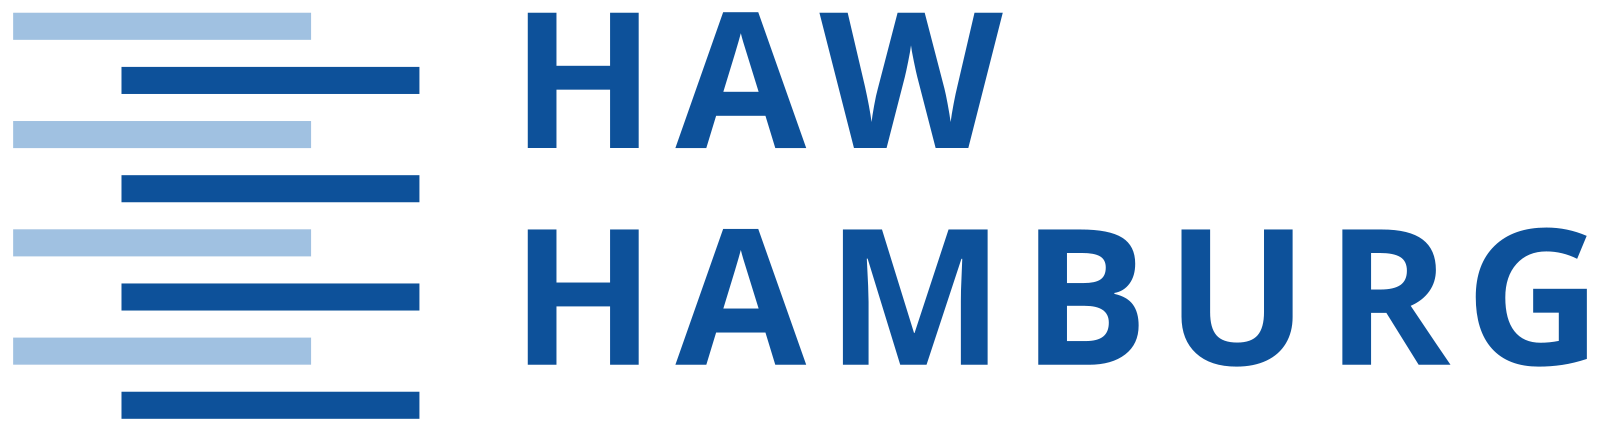
\includegraphics[height=24pt]{HAWLogo}}    % HAW Logo in Kopfzeile einfügen
\lhead{Bussysteme und Sensorik}  % Beschreibung in Kopfzeile

\renewcommand{\footrulewidth}{0.4pt}    % Linie in Fußzeile einfügen
\rfoot{\thepage}    % Seitenzahlen einfügen
\lfoot{Department Informations- und Elektrotechnik}   % Fusszeile linksbündig

\begin{document}
%Titelseite
\begin{titlepage}

  \begin{figure}
    \centering
    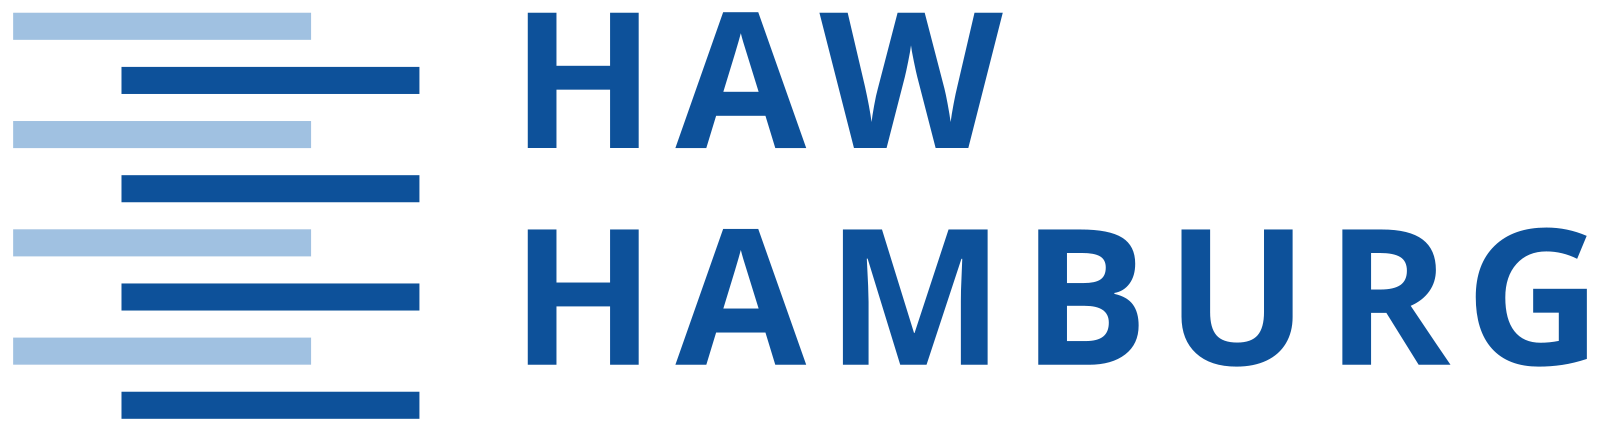
\includegraphics[height=2.5cm]{HAWLogo}
  \end{figure}

  \vspace*{2cm}
  \centering
  {\scshape\Large Bussysteme und Sensorik \par}
  \vspace{1cm}
  {\scshape\LARGE Entwicklung eines Hubs zur Erfassung und graphischen Darstellung von Sensordaten \par}
  \vspace{0.5cm}
  {\scshape\large Wintersemester 2023/2024 \par}
  \vspace{5cm}

  \raggedright
  Ausarbeitung von:

  \vspace{0.5cm}
  Lasse Kelling \\
  2590639

  \vspace{0.2cm}
  Fabian Schmalenbach \\
  2514071

  \vspace{0.5cm}
  Abgabedatum: 24.01.2024

  \vspace{0.5cm}
  Prüfer: Prof. Dr. R. Fitz



\end{titlepage}

\newpage
\addtocontents{toc}{\protect\thispagestyle{empty}}
\tableofcontents
\thispagestyle{empty}
\newpage

\setcounter{page}{1}    % Seitenzähler sicherheitshalber zurücksetzen

\section{Projektbeschreibung}
\label{sub:projektbeschreibung}

Ziel des Projekts ist die Entwicklung eines Sensorhubs, der Sensordaten erfasst und auf einem Display darstellt.
Bei den Sensoren handelt es sich in erster Linie um Umweltdaten, die aktuelle Parameter der Umgebung erfassen.
Das Projekt kann daher grob mit einer Wetterstation verglichen werden. Zusätzlich zu den Sensordaten kann der Sensorhub
die aktuelle Zeit und eine Wettervorhersage über das DCF77-Signal empfangen. 

\subsection{Anforderungen}
\label{subsub:anforderungen}

Es wurden keine verpflichtenden Anforderungen gestellt, das Projekt soll thematisch aber zum Modul
"Bussysteme und Sensorik" passen. Daraus lassen sich für das spezifische Projekt Anforderungen stellen bzw. ableiten:

\begin{itemize}
  \item Verwendung eines oder mehrerer Bussysteme zur Kommunikation zwischen Mikrocontrollern
  \item Nutzung diverser Sensoren mit unterschiedlichen Anbindungen für Vielfältigkeit
  \item Analog zu herkömmlichen Wetterstationen, soll diese ebenfalls über einen Außensensor verfügen
  \item Die Wetterstation soll über eine Wettervorhersage verfügen
  \item Der Sensorhub soll skalier- und erweiterbar sein
\end{itemize}

\noindent
Aus diesen Anforderungen lassen sich direkt Vorgaben für das Projekt ableiten:
\begin{itemize}
  \item Nutzung mehrerer Mikrocontroller, die miteinander über ein Bussystem kommunizieren
  \item Verwendung digitaler Sensoren, die Standardprotokolle wie I2C, SPI oder UART unterstützen
  \item Entwicklung eines Außensensors, der drahtlos mit dem Sensorhub kommunizieren kann
  \item Anbindung des Sensorhubs ans Internet oder Empfang von Wettervorhersagen via Funk (DCF77)
  \item Nutzung ausreichend leistungsstarker Mikrocontroller, die genügend Leistungs- und Peripheriereserven haben, um weitere Geräte anzubinden
\end{itemize}

\section{Systembeschreibung}
\label{sub:systembeschreibung}

\subsection{Systemaufbau}
\label{subsub:systemaufbau}

\begin{figure}[H]
  \centering
  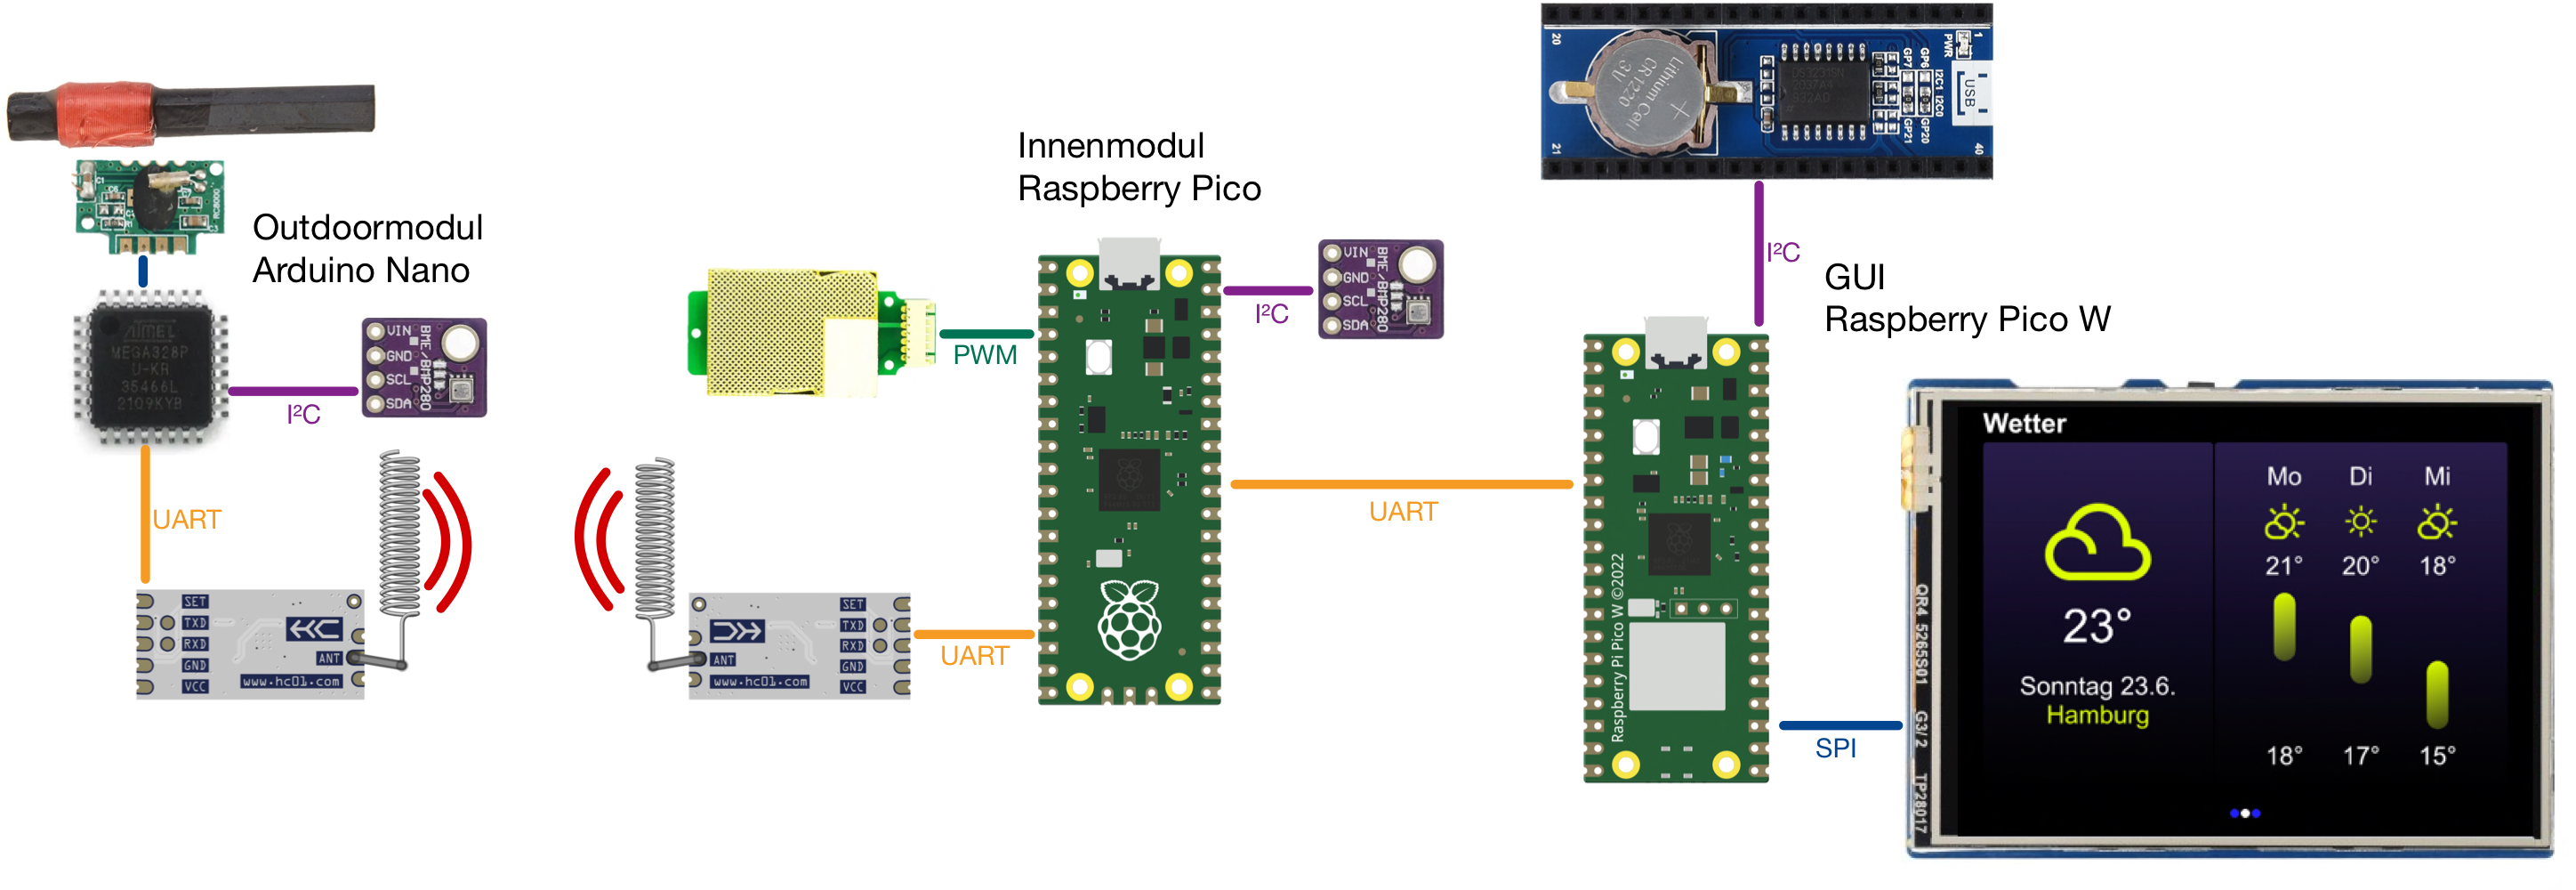
\includegraphics[width = 0.8\textwidth]{Systemuebersicht}
  \caption{Übersicht der Systemkomponenten}
  \label{fig:systemuebersicht}
\end{figure}

Die obige Abbildung \ref{fig:systemuebersicht} zeigt abstrakt alle Komponenten des Systems. Die jeweiligen Komponenten über dem Mikrocontroller Symbol
zeigen jeweils die angeschlossenen Sensoren bzw. Bildschirme. Ebenfalls ist grob die Kommunikation zwischen den Mikrocontrollern erkennbar. 

\vspace{0.2cm}
\noindent
Ganz links ist der Außensensor dargestellt, an den ein Sensor zur Messung von Temperatur, Luftfeuchtigkeit und Luftdruck angeschlossen ist. 
Außerdem verfügt dieser über eine Antenne, um das DCF77-Signal zu empfangen, welches die aktuelle Zeit und eine Wettervorhersage beinhaltet (siehe Abschnitt \ref{subsubsub:dcf77}).
Der Sensor sendet die empfangenen Daten zyklisch per 433 MHz Sender an den Sensorhub. 

\vspace{0.2cm}
\noindent
Der Sensorhub besteht aus zwei Mikrocontrollern, die über eine serielle Schnittstelle (UART) miteinander kommunizieren. Der in Abbildung \ref{fig:systemuebersicht} mittlere Mikrocontroller
empfängt die Daten des Außensensors und leitet diese weiter an den verbundenen Mikrocontroller. Da die Daten zur Wettervorhersage verschlüsselt sind und der Außensensor möglichst
wenig Energie verbrauchen soll, müssen die Daten vom Mikrocontroller entschlüsselt werden. Dazu werden die entsprechenden Datenpakete abgefangen, entschlüsselt und anschließend weitergesendet. 
Der Mikrocontroller verfügt außerdem wie der Außensensor über einen Sensor zur Messung von Temperatur, Luftfeuchtigkeit und Luftdruck (wobei der Luftdruck im Innenraum nicht gemessen wird). 
Zusätzlich ist ein CO2 Sensor verbaut, der die Konzentration im Raum misst. 

\vspace{0.2cm}
\noindent
In der Übersicht ganz rechts ist der Mikrocontroller, der alle Daten empfängt und auf einem Touchdisplay darstellt. Da der Sensor über ein WLAN-Modul verfügt, wäre theoretisch
zusätzlich die Übertragung der Daten per WLAN an einen Server o.ä. möglich, der alle Daten speichert und diese anderen Geräten zur Verfügung stellt. 

\subsection{Sensorik}
\label{subsub:sensorik}

Zur Erfassung der Umweltparameter werden aktuell zwei verschiedene Sensoren eingesetzt. Der BME280 erfasst Lufttemperatur, Luftfeuchtigkeit und Luftdruck. 
Der MHZ19C wird zur Erfassung der CO2 Konzentration im Raum eingesetzt. In den folgenden beiden Abschnitten werden die Sensoren beschrieben. 

\vspace{0.2cm}
\noindent
Das Außenmodul verfügt außerdem über eine 77,5 kHz Empfangsantenne, um das Zeitzeichensignal DCF77 zu empfangen. Daraus lässt sich die aktuelle Zeit ablesen,
außerdem wird eine Wettervorhersage mit übertragen, die ausgewertet wird. 

\subsubsection{BME280}
\label{subsubsub:bme280}

Beim BME280 handelt es sich um einen effizienten Sensor von Bosch, der zur Erfassung von Temperatur, Luftfeuchtigkeit und Luftdruck eingesetzt wird. 
Der Sensor verfügt über ein I2C und SPI Interface.
Beim zyklischen Auslesen aller Sensordaten mit 1 Hz liegt die Stromaufnahme laut Datenblatt bei 3,6 $\mu$A, weshalb sich der Sensor ideal für die Anwendung in Sensormodulen mit Batteriebetrieb eignet. 

Der Sensor verfügt über die folgenden Messbereiche:
\begin{itemize}
  \item Temperatur: -40°C - +85°C ($\pm$ 0,5°C)
  \item Luftfeuchtigkeit: 0 - 100\% rel. Feuchtigkeit ($\pm$ 3\%)
  \item Druck: 250 - 1250 hPa ($\pm$ 1 hPa)
\end{itemize}

\noindent
Mit diesen Spezifikationen eignet sich der Sensor für die Anwendung im Innen- und Außenbereich. 

\noindent
Für das Projekt wird ein Sensorshield verwendet, welches nur den I2C Bus herausführt. Die Kommunikation mit dem Sensor erfolgt daher über I2C. 

\subsubsection{MHZ19C}
\label{subsubsub:mhz19c}

Der MHZ-19C ist ein Infrarot CO2-Sensor, der die CO2 Konzentration mittels nicht-dispersiver Infrarot-Spektroskopie misst. Dabei wird zyklisch mit einer Infrarotlampe
und einem Photosensor die CO2-Konzentration anhand der Reflexion des Lichts durch CO2 Partikel gemessen. 
Der Sensor verfügt über einen Messbereich von 400-5000 ppm, wobei die Genauigkeit $\pm$ 40ppm + 5\% des Messwerts beträgt. 
Da NDIR Sensoren zum Messwertdrift neigen, verfügt der Sensor über eine automatische Kalibrierung, die alle 24 Stunden erfolgt. Der Sensor ist daher für den Dauerbetrieb ausgelegt
und sollte dauerhaft aktiv sein. 
Die Aufheizzeit des Sensors beträgt eine Minute. 

\noindent
Der Sensor ist über eine UART-Schnittstelle konfigurier- und auslesbar, außerdem verfügt er über einen PWM Ausgang. 

\subsubsection{DCF77}
\label{subsubsub:dcf77}

Bei DCF77 handelt es sich um einen Zeitzeichensender in der Nähe von Frankfurt am Main, welcher mit einer Trägerfrequenz von 77,5 kHz ein Zeitsignal überträgt. 
Das Signal ist europaweit empfangbar und wird von den meisten Funkuhren als Referenzsignal verwendet.  

\noindent
Die Datenübertragung erfolgt durch einfache Amplitudenmodulation, indem die Amplitude für eine Dauer von 100 ms (Bit 0) oder 200 ms (Bit 1) auf 25\% der Ausgangsamplitude abgesenkt wird. 
Damit wird eine Bitrate von 1 Bit pro Sekunde erreicht. 

\begin{figure}[H]
  \centering
  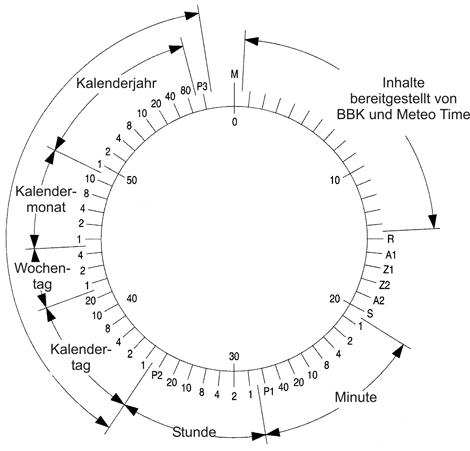
\includegraphics[width=0.7\textwidth]{dcf77Code}
  \caption{Kodierungsschema der DCF77 Zeitinformationen \\
           \url{https://www.ptb.de/cms/ptb/fachabteilungen/abt4/fb-44/ag-442/verbreitung-der-gesetzlichen-zeit/dcf77/zeitcode.html}}
  \label{fig:dcf77Schema}
\end{figure}

\noindent
Abbildung \ref{fig:dcf77Schema} zeigt die Kodierung aller Datenbits innerhalb einer Minute. Daraus ist erkennbar, dass ein Datenpaket 59 Bits lang ist und
die Übertragung eine Minute dauert. Ein Paket beginnt zu jeder neuen Minute. In der letzten Sekunde einer Minute erfolgt keine Absenkung des Trägers, sodass anhanddessen
das Ende eines Pakets abgeleitet werden kann. 

\vspace{0.2cm}
\noindent
Die neue Minute beginnt mit dem nullten Bit, das immer den Wert null hat. Darauf folgen 14 Bits mit verschlüsselten Wetterinformationen der Firma MeteoTime.
Diese werden im nächsten Abschnitt weiter beschrieben. \\
Bit 15 (R) ist ein Rufbit, dass zur Alarmierung der PTB Mitarbeiter dient, wenn Unregelmäßigkeiten vorliegen. \\
Bit 16 (A1) zeigt an, dass am Ende der Stunde ein Wechsel von Sommer- zu Winterzeit stattfindet. \\
Bit 17 (Z1) ist eine Flag für die Sommerzeit. \\
Bit 18 (Z2) ist eine Flag für die Winterzeit. \\
Bit 19 (A2) zeigt an, dass am Ende der Stunde eine Schaltsekunde eingefügt wird. \\
Bit 20 (S) markiert den Beginn der Zeitinformationen und hat den Wert eins. 

\vspace{0.2cm}
\noindent
Wie schon aus der Abbildung hervorgeht, werden in den restlichen Sekunden Informationen zu Zeit und Datum übertragen, Minute, Stunde und Datum haben jeweils ein
Paritätsbit eingefügt, um Fehler erkennen zu können. Eine Fehlerkorrektur ist damit allerdings nicht möglich. 

\subsubsubsection{MeteoTime}
\label{subsubsubsub:meteotime}

MeteoTime versendet versendet pro Minute 14 Bits mit Wetterinformationen, die von lizensierten Geräten entschlüsselt- und verwendet werden können. 
Ein Informationspaket besteht aus 42 Bits und benötigt für die Übertragung somit drei Minuten. Ein Tag ist in fünf Abschnitte unterteilt, in denen
unterschiedliche Informationen übertragen werden. Da die Wettervorhersage 90 Regionen abdeckt, wird jede Vorhersage nur täglich einmal übertragen. \\
Es gilt folgende Aufteilung (MEZ, bei MESZ eine Stunde später): \\
23:00 Uhr - 04:59 Uhr: Aktueller Tag \\
05:00 Uhr - 10:59 Uhr: Folgender Tag \\
11:00 Uhr - 16:59 Uhr: Darauffolgender Tag \\
17:00 Uhr - 19:59 Uhr: Darauffolgender Tag \\
20:00 Uhr - 22:59 Uhr: Zusatzregionen mit 2-Tages Prognose. 

\vspace{0.2cm}
\noindent
Von den 90 Regionen erhalten 60 die viertägige Vorhersage, die restlichen 30 Regionen erhalten nur eine 2-Tages Vorhersage. \\
Innerhalb eines sechsstündigen Übertragungszeitraums werden für jede Region nacheinander die Höchst- und Tiefstwerde übertragen.

\noindent
Die Wettervorhersagen decken große Regionen ab, weshalb diese etwas ungenau sind. \\
Für Hamburg ist beispielsweise die Region Bremerhaven zugeteilt, der Bereich deckt alles vom westlichen Schleswig-Holstein bis zum Nordwesten der Niederlande ab. \\
Um im Fall eines Lesefehlers trotzdem eine Wettervorhersage anzeigen zu können, werden Ausweichzonen genutzt, dessen Wetterdaten stattdessen angezeigt wird. Schlägt
der Empfang für die Region Bremerhaven fehl, wird ausweichend die Vorhersage für Hannover übernommen. Werden auch diese Daten nicht korrekt empfangen, wird die dritte
Ausweichregion Rostock genutzt. 

\vspace{0.3cm}
\noindent
Für die Entschlüsselung der Wetterinformationen ist ein Dekodier-IC notwendig, welches vermutlich aus rückgekoppelten Schieberegistern besteht, um die Daten zu dekodieren. \\
Beim IC handelt es sich um das Modell HKW581 der Firma HKW, die auch Betreiber des MeteoTime Dienstes ist. Der IC ist nur in einem MSOP8 Format erhältlich (SMD).

\begin{figure}[H]
  \centering
  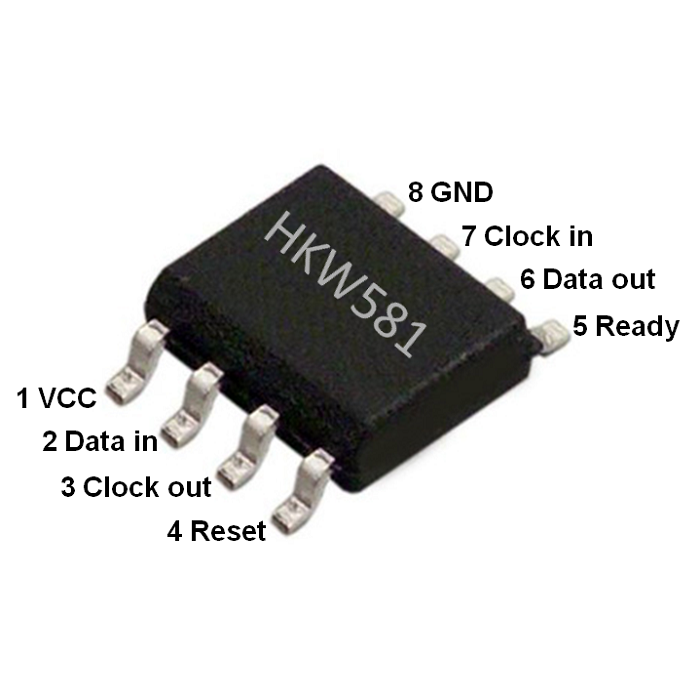
\includegraphics[width = 0.2\textwidth]{HKW5811}
  \caption{Dekodier-IC zum Entschlüsseln der Wettervorhersagen}
  \label{fig:hkw581}
\end{figure}

\noindent
Der IC verfügt über acht Pins, davon sind neben den Pins zur Spannungsversorgung und Daten Ein- und Ausgabe auch ein Clock IN und Clock OUT Pin vorhanden, damit die Bits
taktsynchron ein- bzw. ausgelesen werden. Beim Einlesen der Daten folgt das Clock OUT Signal dem Clock IN Signal, um anzuzeigen, dass die Erfassung des Bits erfolgreich war. 
Nachdem 82 Bits übertragen wurden, wird das Clock OUT Signal invertiert, bis alle Daten vom IC ausgelesen wurden. 
Neben einem Resetpin gibt es außerdem einen Ready Pin, der anzeigt, dass der IC betriebsbereit ist. Anscheinend braucht der IC eine Aufwärmphase. 

\vspace{0.2cm}
\noindent
Als Eingabedaten benötigt der IC einen 82 Bit langen Datenstream, der sich wie folgt zusammensetzt:
\begin{itemize}
  \item Meteopaket 1 (14 Bit)
  \item Meteopaket 2 (14 Bit)
  \item Meteopaket 3 (14 Bit)
  \item Minute des ersten Pakets (aufgefüllt von 7 auf 8 Bit)
  \item Stunde des ersten Pakets (aufgefüllt von 6 auf 8 Bit)
  \item Kalendertag (aufgefüllt von 6 auf 8 Bit)
  \item Monat (5 Bit)
  \item Wochentag (3 Bit)
  \item Jahr (8 Bit)
\end{itemize}

\noindent
Als Ausgabe erhält man einen 22 Bit langen Datenstream mit den Wetterinformationen. Je nachdem, ob gerade ein Paket mit Höchst- oder Tiefstwerten gesendet wurde, 
ergeben sich unterschiedliche Informationen:

\vspace{0.2cm}
\noindent
Höchstwerte:
\begin{itemize}
  \item Wetter Tag (4 Bit)
  \item Wetter Nacht (4 Bit)
  \item Schweres Wetter (4 Bit)
  \item Niederschlagswahrscheinlichkeit(3 Bit)
  \item Wetteranomalie Tag (1 Bit)
  \item Temperatur Tag (6 Bit)
\end{itemize}

\vspace{0.2cm}
\noindent
Tiefstwerte:
\begin{itemize}
  \item Wetter Tag (4 Bit)
  \item Wetter Nacht (4 Bit)
  \item Windrichtung (4 Bit)
  \item Windstärke (3 Bit)
  \item Wetteranomalie Nacht (1 Bit)
  \item Temperatur Nacht (6 Bit)
\end{itemize}

\noindent
Die ausgegebenen Zahlenwerte sind wiederum einer Bezeichnung zugeordnet (z.B. Wetter Tag = 3 entspricht vorwiegend bewölkt).

\newpage
\subsection{Kommunikation}
\label{subsub:kommunikation}

Die Kommunikation zwischen den Mikrocontrollern erfolgt sowohl kabelgebunden, als auch drahtlos. Für die kabelgebundene Kommunikation wird UART mit einer Baudrate
von 115200 bd genutzt. Die Drahtloskommunikation erfolt über einen 433 MHz Transmitter und Receiver, die jeweils im Halbduplexverfahren wie eine UART Schnittstelle
genutzt werden können. 

\subsubsection{Funkstrecke}
\label{subsubsub:funkstrecke}

Bei den Funkmodulen handelt es sich um "HC-12 Wireless RF communicatio module V2.4" Module. Diese versprechen eine Übertragungsdistanz von bis zu 1800 m
und eine einfache Ansteuerung über UART. \\
Die Module können jeweils sowohl Daten senden. 
Die Sendeleistung beträgt bis zu 100 mW und es können 100 verschiedene, einstellbare Kanäle genutzt werden (433,4 MHz bis 473 MHz). Die Baudrate ist zwischen 
1200 bps und 115200 bd wählbar. 

\vspace{0.2cm}
\noindent
Aktuell wird eine Baudrate von 9600 bd verwendet, um ein gutes Mittel zwischen Distanz und Geschwindigkeit zu erzielen. 

\vspace{0.5cm}
\noindent
Aufgrund der geltenden Bestimmungen in Deutschland darf nur mit maximal 10 mW gesendet werden, auch ist der wählbare Frequenzbereich teilweise nicht legal.
Es können nur die Kanäle 1 bis 4 genutzt werden. 

\subsubsection{Datenpakete}
\label{subsubsub:datenpakete}

Je nach übertragener Information werden unterschiedliche Datenpakete verwendet, die zur Identifikation jeweils mit einem 4-Byte langen Identifier ausgestattet sind. \\
Aktuell gibt es fünf verschiedene Identifier:
\begin{itemize}
  \item 'IBME' Internal BME
  \item 'EBME' External BME
  \item 'CO2.' Co2 Konzentration
  \item 'TIME' Aktuelle Zeit
  \item 'MTEO' Wettervorhersage
\end{itemize}

\noindent
Die Datenpakete haben unterschiedliche Längen und sind in Form von Structs in C definiert. Zum Senden der Daten werden diese dann in char arrays umgewandelt. \\
Da die Structs unterschiedliche Datentypen beherbergen, fügt der Compiler normalerweise Padding Bytes ein, um gleichmäßige Addressabstände zu gewährleisten. 
Für die Verarbeitung und Übertragung der Datenpakete ist dies aber problematisch, weil beispielsweise die zu sendenden Datenpakete größer als nötig sind. 
Aus diesem Grund werden die Structs mit dem Attribut packed versehen, damit auf Padding Bytes verzichtet wird. 
Alle Datenpakete sind im folgenden dargestellt:

\newpage
\lstinputlisting[language=C, caption=Datenpakete]{dataTypes.h}

\noindent
Wie man im obigen Listing sieht, haben alle Datenpakete zusätzlich eine CRC-8 Prüfsumme, die bei der drahtlosen Datenübertragung 
zur Prüfung des Pakets verwendet wird. Bei der kabelgebundenen Datenübertragung zwischen beiden Mikrocontrollern
auf dem Innenmodul wird auf eine Prüfsumme verzichtet. 

\subsubsection{Übertragungsfehler}
\label{subsubsub:uebertragungsfehler}

Da die Meteotime Pakete jeweils nur einmal gesendet werden und ein Paketverlust bei der 433 MHz Datenübertragung problematisch wäre, wird, wie schon erwähnt, eine Prüfsumme
berechnet und übertragen und auf der Empfängerseite auf Richtigkeit überprüft. Ist die Prüfsumme fehlerhaft, sendet der Empfänger einen Retransmission-Befehl an den Sender.
Im folgenden ist die sowohl die fehlerfreie Übertragung von Paketen als auch die Übertragung mit mehrfacher Retransmission dargestellt. 

\begin{figure}[H]
  \centering
  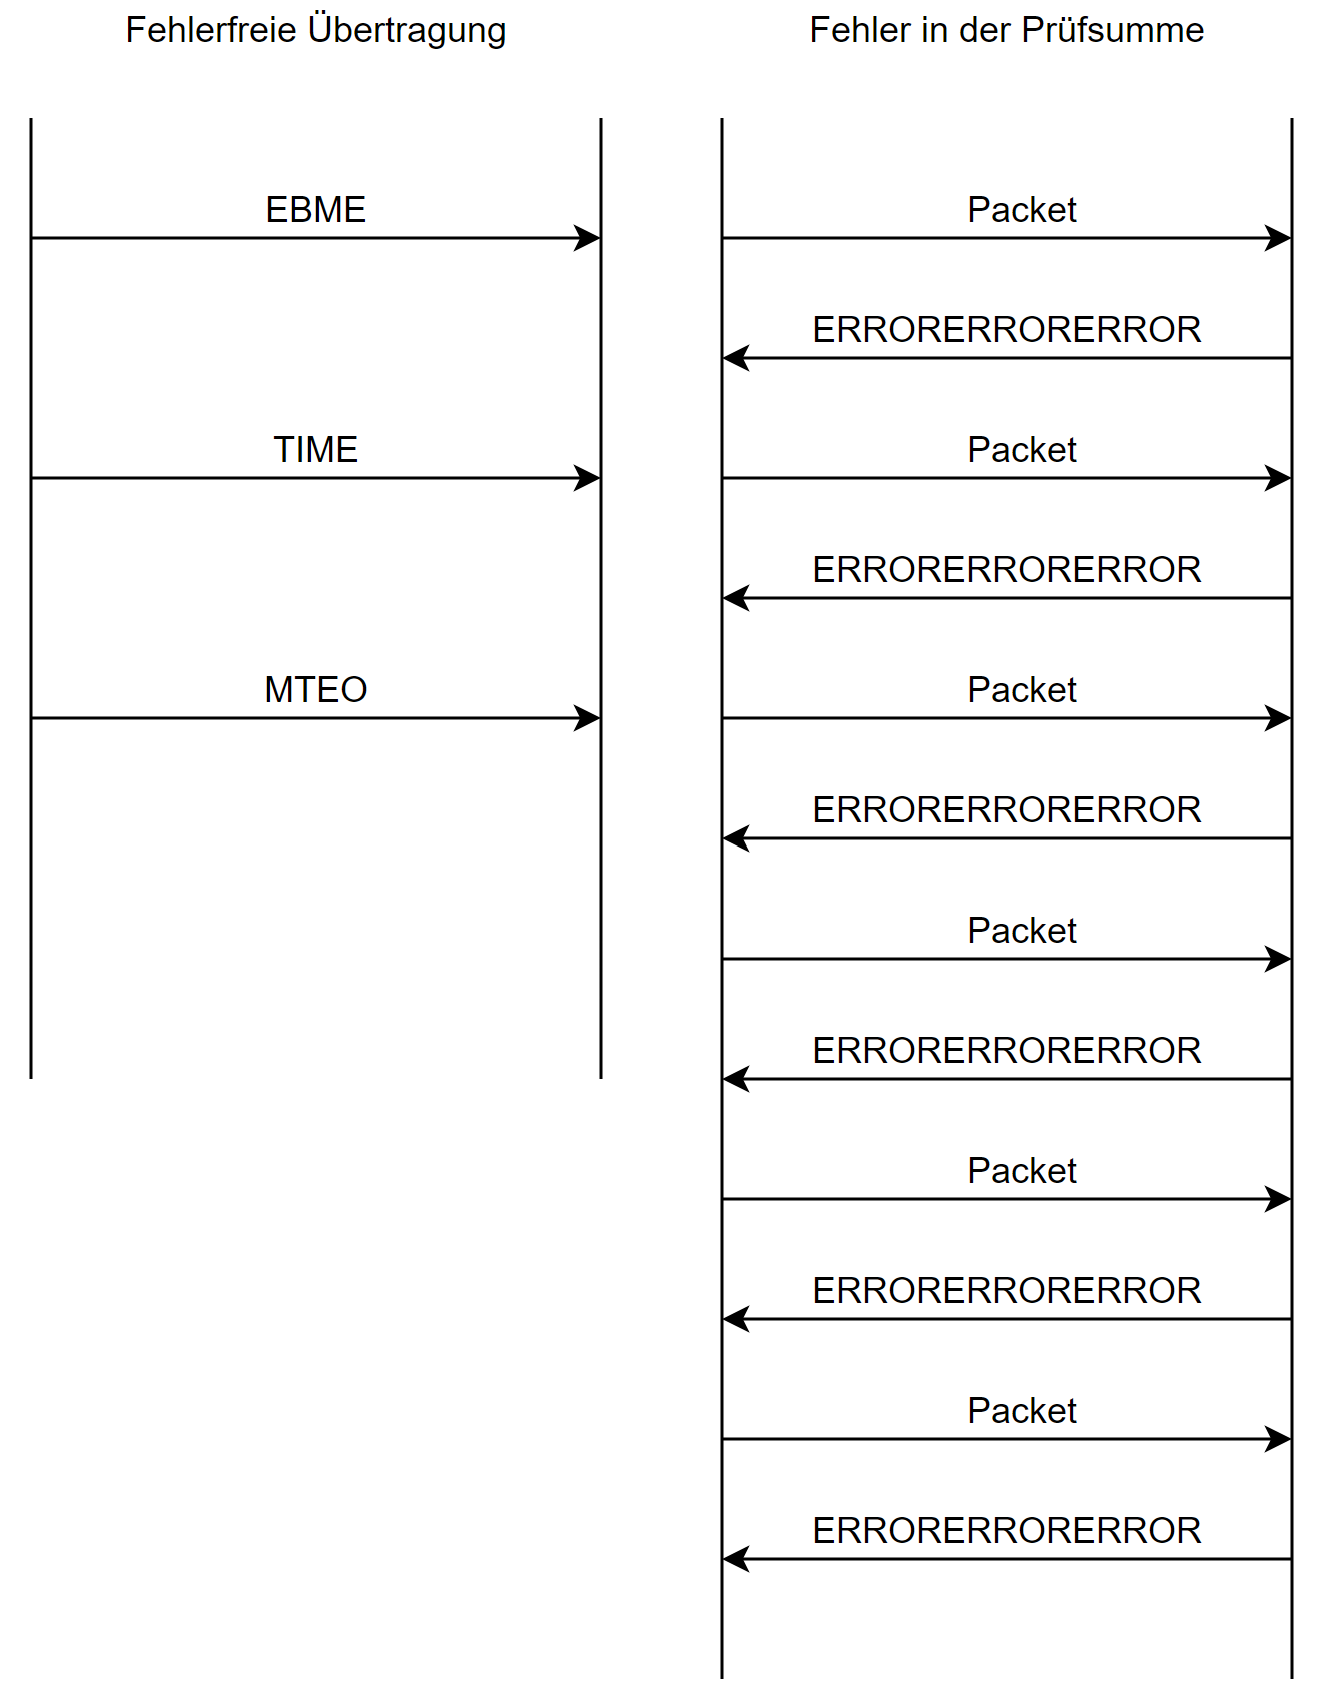
\includegraphics[width=0.6\textwidth]{Kommunikation}
  \caption{Kommunikationsablauf zwischen Innen- und Außenmodul ohne und mit Übertragungsfehler}
  \label{fig:kommunikation}
\end{figure}

\noindent
Aus Abbildung \ref{fig:kommunikation} geht hervor, dass das Innenmodul den String ``ERRORERRORERROR'' an das Außenmodul sendet, wenn die Prüfsumme vom vorher gesendeten Paket
fehlerhaft ist. Der String wurde so gewählt, damit eventuell zufällig empfangene einzelne Bits anderer Quellen ignoriert werden und bei schlechtem Empfang zumindest ein paar Bytes
empfangen werden. Das Außenmodul reagiert mit einer Retransmission, wenn es fünf Bytes empfangen hat. \\
Die Zahl der Retransmissions ist auf fünf begrenzt, danach verwirft das Außenmodul das Paket. \\
Ein Retransmission Paket muss vom Innenmodul innerhalb von drei Sekunden an das Außenmodul gesendet werden, andernfalls nimmt das Außenmodul an, dass die Übertragung
erfolgreich war. 

\section{Modulbeschreibung}
\label{sub:modulbeschreibung}

\subsection{Sensormodul extern}
\label{subsub:sensorModul_ext}

Das externe Sensormodul soll im Außenbereich angebracht werden und möglichst effizient per Batterie betrieben werden können. \\
Wie schon aus den vorherigen Abschnitten hervorgeht, verfügt das Modul über einen BME280 für Temperatur, Luftfeuchtigkeit und Luftdruck
und eine Antenne zum Empfang des DCF77 Signals. Die empfangenen Daten werden dann zyklisch via 433 MHz an den Sensorhub gesendet. Die DCF77 Antenne
ist im Außenmodul untergebracht, weil das Signal sehr anfällig für Störungen durch elektrische Geräte oder Abschirmung durch Metalle ist, 
die vorallem im Innenbereich vorkommen. Im Außenbereich ist der Empfang besser. 

\vspace{0.2cm}
\noindent
Für den DCF77 Empfang wird ein Shield verwendet, das eine auf 77,5 kHz abgestimmte Antenne hat und das Signal filtert und in saubere TTL Pegel umwandelt.
Im Mikrocontroller wird eine Bibliothek verwendet, die einen Interrupt mit Trigger auf steigende- und fallende Taktflanke verwendet, um die Dauer der Absenkung
des Trägersignals zu messen. In der letzten Sekunde einer Minute findet keine Absenkung statt, anhanddessen wird das Ende eines Datenpakets ermittelt.
Da in der letzten Sekunde einer Minute keine Absenkung stattfindet, kann anhanddessen das Ende eines Datenpakets ermittelt werden. 
Zum Ende jeder Minute wird das Paket auf Gültigkeit überprüft. Dazu werden zum einen die Paritätsbits auf den richtigen Wert überprüft, außerdem
wird geprüft, ob die Flag für die Sommerzeit den gegenteiligen Wert der Flag für die Winterzeit hat. 
Ist die Überprüfung in Ordnung, wird das Datenpaket für die Zeit aus dem erhaltenen Zeitstempel zusammengesetzt und versendet. \\
Alle drei Minuten ist außerdem ein Meteotime Paket fertig und kann durch den Dechiffrier-IC entschlüsselt werden. 

\vspace{0.2cm}
\noindent
Ein Ablaufdiagramm zur Beschreibung der Software ist im Anhang in \hyperref[pdf:ablaufExtern]{Abbildung \ref{pdf:ablaufExtern}} zu finden. Es wird zyklisch geprüft, ob ein Zeit, Meteo oder Sensorpaket
versendet werden kann und ob die Übertragung fehlerfrei abgelaufen ist. Die Dekodierung der Wetterdaten erfolgt in der Klasse Meteo, im Dekodierprozess nacheinander
jedes Bit des Pakets in den Decoder geschrieben und anschließend der Bitstream aus dem IC gelesen. War die Entschlüsselung der Daten fehlerhaft, gibt der Decoder den String
``100000000000000000000100'' aus. 

\vspace{0.2cm}
\noindent
Als Mikrocontroller wurde in ersten Tests zunächst ein ESP8266 verwendet. Da dieser einen relativ hohen Energieverbrauch von ca. 20 mA hat und zudem für
den Anwendungszweck leistungstechnisch überdimensioniert ist, wurde als Alternative ein energiesparender MSP430G2553 gewählt, der bei 1 MHz Takt nur
230 $\mu$A verbrauchen soll und sowohl einen UART, als auch I2C Bus hat. Damit wäre ein langfristiger Betrieb mit Batterie möglich gewesen. 
Aus Zeitgründen und wegen der fehlenden Portierungsmöglichkeit des ESP8266 Codes auf den MSP430 wurde stattdessen ein Arduino Nano gewählt, einen ATmega328p
Mikrocontroller als Basis verwendet. Modifiziert man einige Teile am Board, lässt sich der Stromverbrauch laut einiger Quellen auf ca. 5 mA drosseln. 

\subsubsection{Platinenentwurf}
\label{subsubsub:platinenentwurfExtern}

Für beide Module wird eine Platine angefertigt, um das Projekt auch in der Realität anwendbar zu machen. Das Außenmodul ist für den Batteriebetrieb konzipiert
und daher mit einigen Aktivbauteilen ausgestattet. Die Bauteile wurden zusammen mit der Platine bei JLCPCB bestellt und dort bestückt. 

\subsubsubsection{Schaltplan}
\label{subsubsubsub:schaltplanExtern}

Der Schaltplan ist im Anhang in \hyperref[pdf:schaltplanExtern]{Abbildung \ref{pdf:schaltplanExtern}} dargestellt. Zentraler Bestandteil ist dabei der Mikrocontroller. 
Für die Spannungsregulierung werden zwei Schaltregler verwendet, die 5 V und 3,3 V aus der Batteriespannung generieren. Beide Schaltregler arbeiten bis zu einer Minimalspannung
von ca. 0,7 V, die angeschlossene Batterie kann also fast vollständig genutzt werden. Beide Schaltregler vertragen maximal 5,5 V am Eingang, weshalb als Spannungsquelle
drei Alkaline Batterien in Serie dienen sollen, die eine Spannung von ca. 4,5 V bereitstellen. 
Die Anschlusskabel des Batteriefachs werden an die Platine gelötet, dafür wurden je 4x4 mm große Pads gewählt. 

\vspace{0.2cm}
\noindent
An den Mikrocontroller sind wie vorher beschrieben der HKW581 IC, ein BME280, die 433 MHz- und die DCF77-Antenne angeschlossen. Zu Entwicklungszwecken sind einige 
Zusatzanschlüsse vorhanden, um Modifikationen möglich zu machen. \\
Der HKW581 ist im MSOP8 Format und damit relativ klein. Um den IC schon bei vorherigen Testaufbauten auf dem Steckbrett nutzen zu können, wurde dieser auf einen Adapter
gelötet, der die Anschlusspins auf einfache THT Pins adaptiert. Um den IC zu schonen, wird der Adapter auf der Platine verbaut. Zusätzlich besteht aber die Möglichkeit, 
später darauf zu verzichten und das Bauteil direkt auf der Platine festzulöten. Diese Lösung findet sich ebenso auf dem später beschriebenen Innenmodul wieder, falls
auf das Außenmodul verzichtet werden soll. \\
Als BME280 soll in erster Linie ein fertiges Shield zum Aufstecken verwendet werden, da der private Bestand davon wesentlich höher ist. Zusätzlich kann manuell aber auch
direkt ein BME280 auf die Platine gelötet werden. Die entsprechenden Bauteile sind nicht platziert. \\
Es können zwei verschiedene Arten von DCF77 Antennen an den Mikrocontroller angeschlossen werden. Dabei wird unterschieden zwischen Shields mit drei- und vier Anschlüssen. 
Die Shields mit vier Anschlüssen verfügen zusätzlich über einen PON (Power On) Pin, über den das Modul an- und ausgeschaltet werden kann. Der Pin ist normalerweise low
active und wird daher auf Masse gelegt. 

\subsubsubsection{Platine}
\label{subsubsubsub:platineExtern}

Die Platine ist im Anhang in \hyperref[pdf:platineExtern]{Abbildung \ref{pdf:platineExtern}} und \hyperref[fig:platineExtern3D]{Abbildung \ref{fig:platineExtern3D}} dargestellt. Es handelt sich um eine einfache 2-Layer Platine mit Ground Plane
auf der Unterseite. An der Oberseite sind Befestigungsmöglichkeiten für die DCF77 Antenne vorgesehen (dort ist auch keine Ground Plane mehr, um Abschirmungen zu vermeiden). 
Im Test hat sich allerdings herausgestellt, dass die Antenne nichts empfängt, wenn sie auf der Platine angebracht ist. 

\newpage
\subsection{Modul intern}
\label{subsub:modulInt}

\subsubsection{Sensormodul}
\label{subsubsub:sensormodulInt}

Das interne Sensormodul darf im Gegensatz zum externen Modul mehr Energie verbrauchen, da es mehr Daten verarbeiten muss und über einen Netzanschluss verfügt. 
Das Modul empfängt die über 433 MHz gesendeten Daten und liest zusätzlich zyklisch den BME280 und CO2 Sensor aus.

\vspace{0.3cm}
\noindent
Als Mikrocontroller wird ein Raspberry Pi Pico verwendet, der mit zwei kernen Multiprocessing erlaubt und damit die Reaktionszeiten beschleunigt. Der Mikrocontroller
verfügt über zwei UART Busse und zwei I2C Busse. Die beiden UART Busse werden für die Kommunikation mit dem Grafikmodul und dem 433 MHz Modul verwendet.

Der verwendete CO2 Sensor verfügt zwar auch über eine UART-Schnittstelle, die zur Verfügung stehenden UART Emulatoren für den Mikrocontroller lieferten allerdings
falsche Daten. Aus diesem Grund wird der Duty Cycle des zur Verfügung stehenden PWM Pins genutzt. 
Eine Bibliothek für den Sensor liest den PWM Pins automatisch aus und konvertiert den Duty Cycle in eine CO2 Konzentration. Da das Auslesen des PWM Signals insbesondere bei hohen
Konzentrationen recht lang dauern kann, erfolgt dies ausschließlich über den zweiten Kern, der neue Werte global zur Verfügung stellt und dies über eine Flag signalisiert. 

\subsubsection{Grafikmodul}
\label{subsubsub:grafikmodulInt}

Das Grafikmodul wird beim Endprodukt zusammen mit dem \hyperref[subsub:sensormodulInt]{internen Sensormodul} als eine Baugruppe ausgeführt sein.
Hauptziel ist die grafische Aufarbeitung der über UART vom \hyperref[subsub:sensormodulInt]{internen Sensormodul} empfangenen Daten.
Hierfür wird ebenfalls ein Raspberry Pi Pico in der W-Variante eingesetzt.
Diese ist zusätzlich zu den Schnittstellen des Picos W-LAN (IEEE 802.11 b/g/n) und Bluetooth (5.2 LE) fähig, somit kann das Grafikmodul zukünftig ebenfalls die Rolle eines mqtt-Brokers übernehmen und die aufbereiteten Daten online abrufbar machen.
Für diese Aufgaben verfügt das Modul über einen externen RTC-Chip und ein 2,8 Zoll Touchdisplay.

\vspace{0.3cm}
\noindent
Anders als bei den Sensoren wird beim Grafikmodul kein C-Code verwendet sondern ausschließlich in Rust programmiert.
Embedded-Rust folgt dem Motto \textquoteleft safe, fast, concurrent – pick three\textquoteright.
Rust etabliert viele Konzepte, um die typischen Probleme, die mit vergessenen Sonderfällen einhergehen (dangling pointer, use after free, dead-locks, integer-overflow, uvm.) durch ein gutes Typsystem und einen modernen Compiler bereits zur Kompilierzeit auszuschließen.
Ein Embedded-Rust-Projekt, welches erfolgreich kompiliert, wird in der Praxis auf dem Mikrocontroller nie unerwartetes Verhalten aufweisen.
Trotzdem wird noch eine von C-Programmen gewohnte Performance erreicht.

\vspace{0.3cm}
\noindent
Durch die Verwendung von Rust kann ebenfalls die sehr moderne Bibliothek Slint für die graphische Darstellung verwendet werden. Diese kompiliert Slint-Strukturen zu Rust-Quelltext und stellt Schnittstellen bereit, um fertige Pixelbuffer zu erhalten.

\vspace{0.3cm}
\noindent
Slint-Strukturen gliedern sich in components, globals und structs.
Ein Component ist ein auf dem Display anzeigbarer Baustein.
Globals stellen einen Adapter zum Rust-Quelltext dar, da man die Daten dieser sowohl aus dem Slint-Skript, als auch aus dem Rust-Programm verändern kann.
Structs in Slint definieren wie Structs in C oder Rust eigene zusammengesetzte Datentypen.

\lstinputlisting[language=slint, caption=Beispiel eines components globals und structs]{gui.slint}

\vspace{0.3cm}
\noindent
Während Slint das Zeichnen der Grafikbausteine übernimmt, muss sich der selbstgeschriebene Code um folgende Funktionen kümmern:
\begin{itemize}
	\item Initialisierung der Peripherie und Anbindung von Slint
	\item Ansteuerung des RTC Moduls (per I2C)
	\item Übertragung der Pixel an das Display (per DMA SPI)
	\item Übertragung des Touchinputs an den Pico (per DMA SPI)
	\item Übertragung der Sensordaten (per UART)
\end{itemize}

\vspace{0.3cm}
\noindent
Um Rechenleistung einzusparen, ist der Großteil des Programms mithilfe der wfe und sev Anweisungen des Picos (\textbf{W}ait\textbf{F}or\textbf{E}vent und \textbf{S}et/\textbf{S}ignal\textbf{EV}ent) Event-basiert implementiert.
Ein entsprechendes Interrupt wird ausgelöst, wenn
\begin{enumerate}
	\item ein UART-Package vom \hyperref[subsub:sensorModul_int]{internen Sensormodul} empfangen wurde
	\item Bildinhalte sich verändert haben (beispielsweise die Uhrzeit jede volle Sekunde)
	\item der Touchscreen berührt wird
\end{enumerate}

\lstinputlisting[language=rust, caption=Eventloop mit wfe]{eventloop.rs}

\begin{figure}[H]
	\centering
	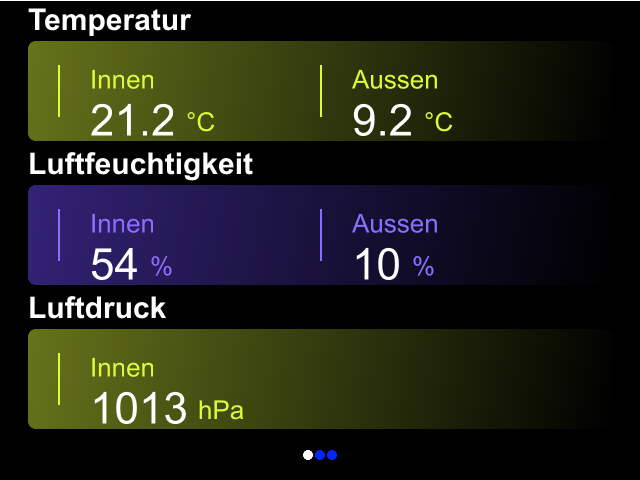
\includegraphics[width=0.8\textwidth]{Overview}
	\caption{Übersichts-Seite des GUI}
	\label{fig:gui-overview}
\end{figure}

\begin{figure}[H]
	\centering
	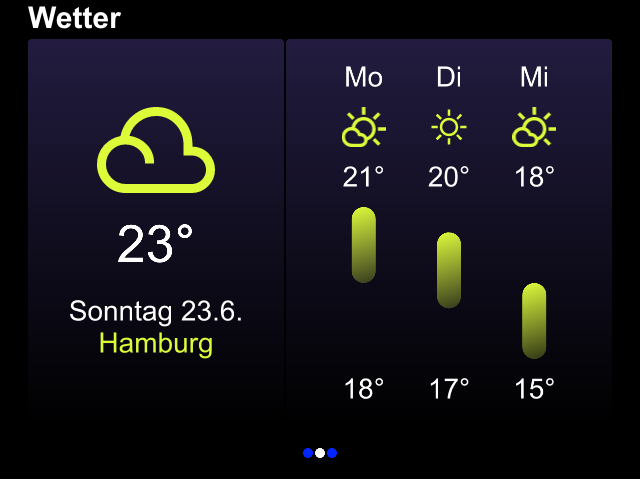
\includegraphics[width=0.8\textwidth]{Weather}
	\caption{Wetter-Seite des GUI}
	\label{fig:gui-overview}
\end{figure}

\subsubsection{Platinenentwurf}
\label{subsubsub:platinenentwurfExtern} 

\subsubsubsection{Schaltplan}
\label{subsubsubsub:schaltplanExtern}

Der Schaltplan ist im Anhang in \hyperref[pdf:schaltplanIntern]{Abbildung \ref{pdf:schaltplanIntern}} dargestellt. Zentraler Bestandteil sind die beiden Mikrocontroller, 
die über eine UART Verbindung miteinander kommunizieren. Der Raspbery Pi Pico W, der das Grafikmodul beherbert, steuert das aufsteckbare Touchdisplay. Zusätzlich wird
ein RTC Shield auf den Mikrocontroller gesteckt, um die aktuelle Zeit speichern zu können und jitter zu minimieren. 
An den Raspberry Pi Pico, der die Sensoren ausliest, sind ein BME280, der CO2 Sensor und die 433 MHz Antenne angebunden. Zusätzlich kann hier ein HKW581 Modul integriert werden, 
dieses befindet sich im aktuellen Aufbau aber auf dem Außenmodul. Wie schon im externen Modul sind Möglichkeiten für das Shield und den Adapter vorbehalten. 
Der HKW581 auf dem internen Modul ist nur sinnvoll, falls auf das Außenmodul verzichtet werden soll (nicht geplant).

\subsubsubsection{Platine}
\label{subsubsubsub:platineExtern}

Die Platine ist im Anhang in \hyperref[pdf:platineIntern]{Abbildung \ref{pdf:platineIntern}} und \hyperref[fig:platineIntern3D]{Abbildung \ref{fig:platineIntern3D}} dargestellt. Es handelt sich um eine einfache 2-Layer Platine mit Ground Plane
auf der Unterseite. Hervorzuheben sind die Befestigungsmöglichkeiten des Displays sowie Bohrlöcher an den Außenseiten zur Befestigung im Gehäuse, o.ä..
Auf der Platine sind zwei Anschlüsse zur Spannungsversorgung der Platine eingeplant, einer führt das Kabel seitlich nach links, der andere nach unten. 
Der Anschluss nach unten kann praktisch sein, wenn die Platine aufgehängt werden sollte. Wird diese hingegen aufgestellt, ist eine seitlich Führung des Kabels nötig. 


\section{Funktionstest}
\label{sub:funktionstest}

Der Funktionstest ist wegen der graphischen Oberfläche auf dem Display nicht ganz einfach zu dokumentieren. 

\subsection{Test der Sensorik}
Da der Raspberry Pi Pico im Gegensatz zu herkömmlichen Arduinos zusätzlich zu den UART Bussen serielle Daten über die USB Schnittstelle übertragen kann, 
sind einfache Print Ausgaben der empfangenen und weitergeleiteten Daten die einfachste Möglichkeit. 

\begin{figure}[H]
  \centering
  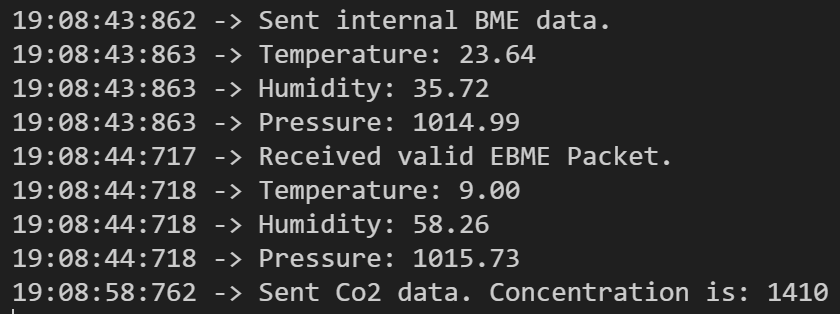
\includegraphics[width=0.8\textwidth]{SensorLog.png}
  \caption{Logausgabe von internen und externen Sensordaten und CO2 Konzentration}
  \label{fig:sensorlog}
\end{figure}

\noindent
Abbildung \ref{fig:sensorlog} zeigt die Logausgabe von BME Daten des externen und internen Sensors und die aktuell gemessene CO2 Konzentration. 
``Received valid EBME Packet'' zeigt an, dass die übertragene Prüfsumme korrekt ist und keine Übertragungsfehler detektiert wurden. 
Die drei Pakete werden anschließend über die UART-Schnittstelle an das Grafikmodul weitergeleitet. 

\vspace{0.2cm}
\noindent
Ebenso werden die übertragenen Zeit- und Meteotimepakete in der Konsole ausgegeben:

\begin{figure}[H]
  \centering
  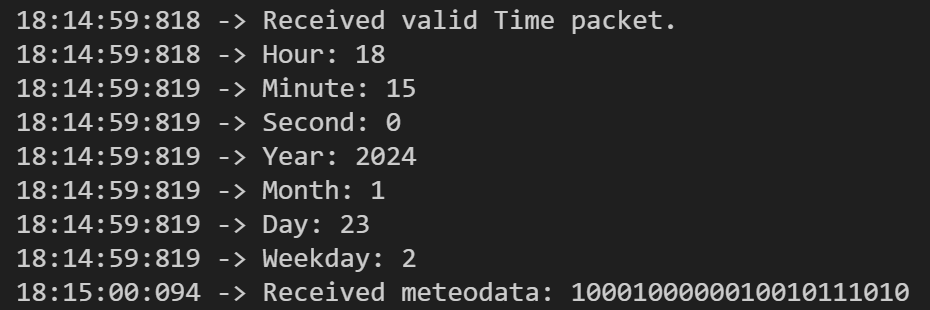
\includegraphics[width=0.8\textwidth]{MeteotimeLog.png}
  \caption{Logausgabe eines Zeit- und Meteotimepakets}
  \label{fig:meteolog}
\end{figure}

\noindent
Ein Meteotime Paket wird nur übertragen, wenn es relevant für die Wetterstation ist (relevante Zone) und, wenn die Ausgabe des Dekodier-ICs fehlerfrei ist. 
Beim hier angezeigten Meteotime Paket handelt es sich um die Höchstwerte für den Tag + 3 für die Region Rostock. Das Paket ist 24 bit lang (die beiden führenden Nullen
werden hier nicht mit angezeigt). 

\vspace{0.2cm}
\noindent
Aus dem Paket lassen sich folgende Informationen ermitteln:

\begin{table}[H]
  \centering
  \begin{tabular}{|l|l|l|l|}
  \hline
  \textbf{Binärwert} & \textbf{Lage}                   & \textbf{Dezimalwert} & \textbf{Beschreibung} \\ \hline
  0010               & Tag                             & 4                    & bedeckt               \\ \hline
  0010               & Nacht                           & 4                    & bedeckt               \\ \hline
  0000               & Wetterextrema                   & 0                    & keine                 \\ \hline
  010                & Niederschlagswahrscheinlichkeit & 2                    & 30\%                  \\ \hline
  0                  & Wetteranomalie                  & 0                    & Nein                  \\ \hline
  101110             & Temperatur                      & 29                   & 7°C                   \\ \hline
  10                 & Dekoderstatus                   & -                    & OK                    \\ \hline
  \end{tabular}
  \caption{Informationen aus dem Meteotime Paket}
  \label{tab:meteopacket}
  \end{table}

\subsection{Test des Grafikmoduls}

\section{Fazit}
\label{sub:fazit}

\newpage
\appendix

\section{Ablaufdiagramm externes Modul}
\label{subapp:ablaufExt}

\begin{figure}[H]
  \centering
  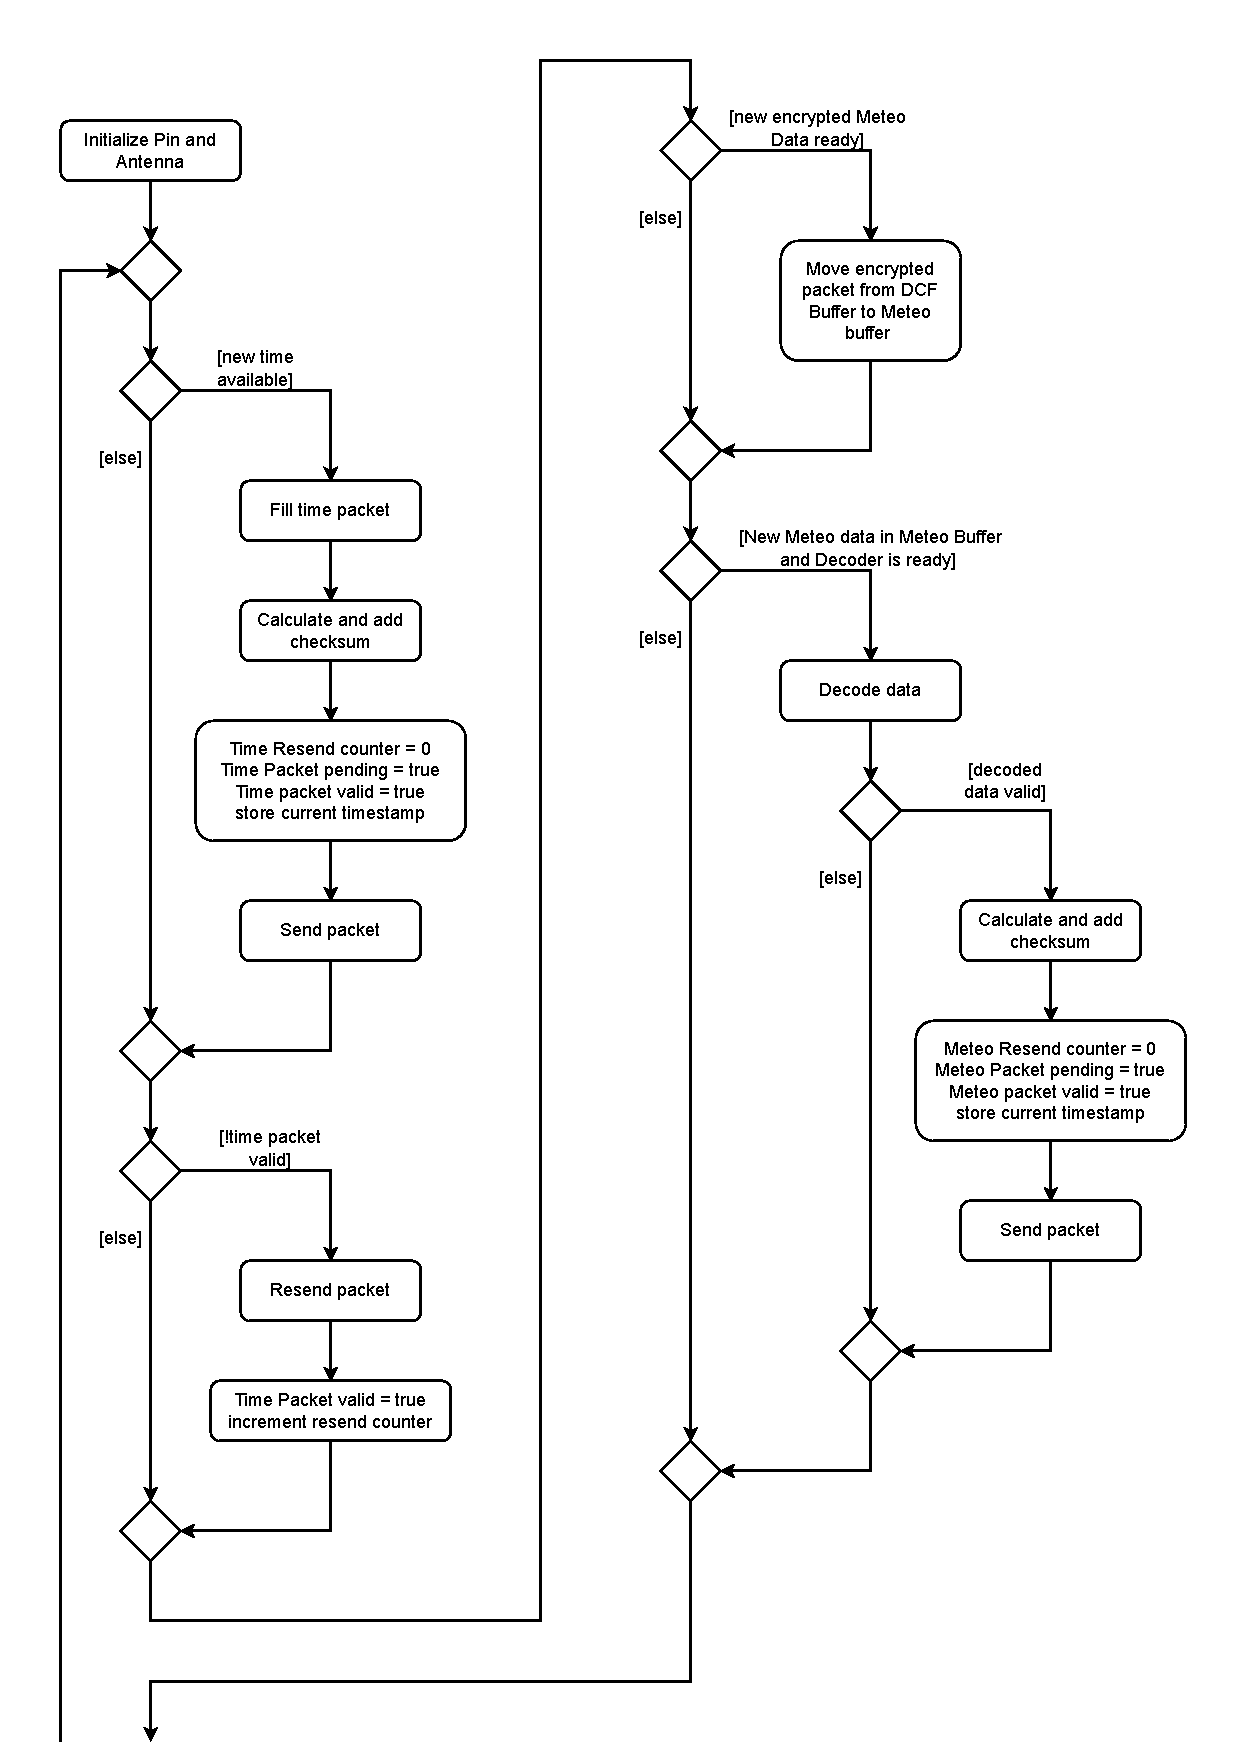
\includegraphics[scale=0.75, page=1]{Ablauf extern.pdf}
\end{figure}

\begin{figure}[H]
  \centering
  \includegraphics[scale=0.75, page=2]{Ablauf extern.pdf}
\end{figure}

\begin{figure}[H]
  \centering
  \includegraphics[scale=0.75, page=3]{Ablauf extern.pdf}
  \caption{Abstraktes Ablaufdiagramm zur Beschreibung des Codes auf dem externen Sensormodul}
  \label{pdf:ablaufExtern}
\end{figure}

\newpage
\section{Schaltplan externes Modul}

\begin{figure}[H]
  \centering
  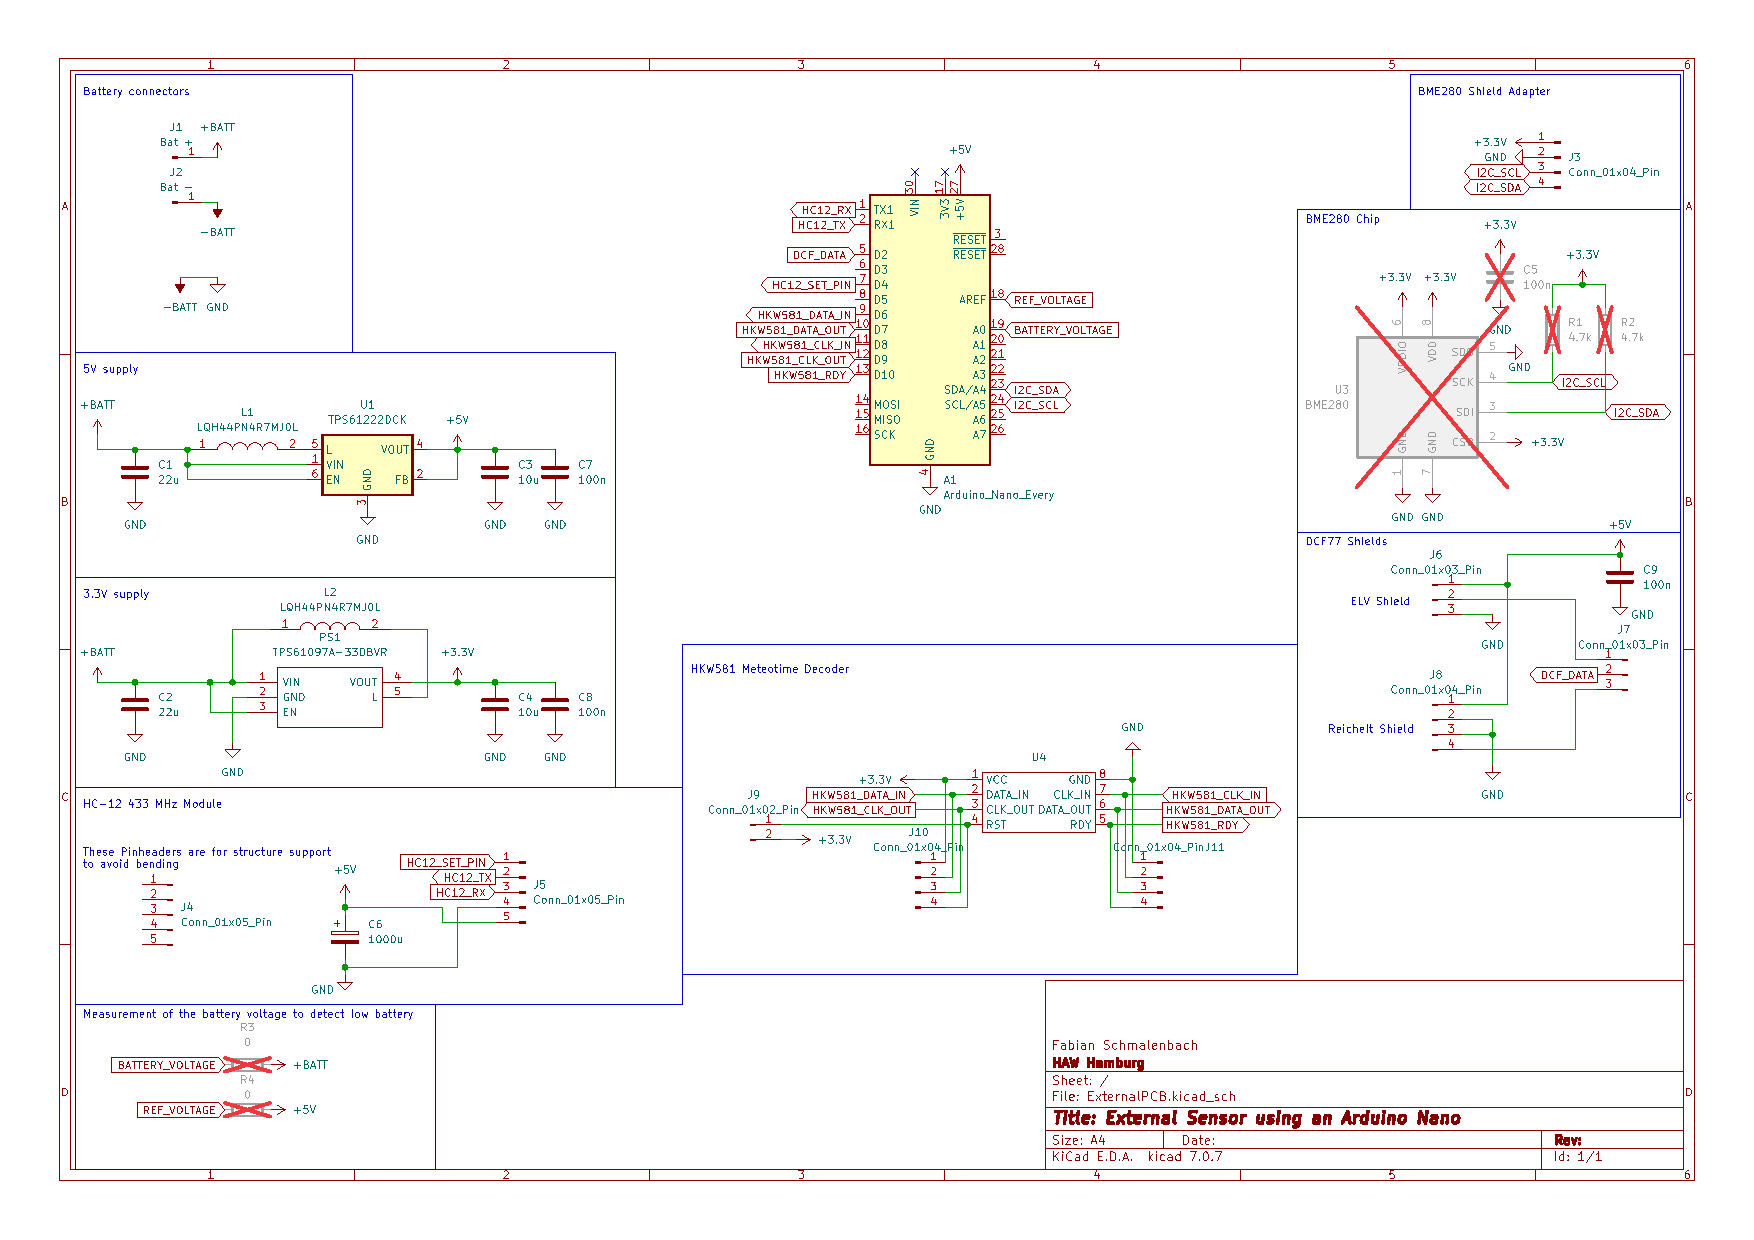
\includegraphics[scale=0.7, page=1, angle=90]{../pcbs/ExternalPCB/ExternalPCB.pdf}
  \caption{Schaltplan des externen Moduls}
  \label{pdf:schaltplanExtern}
\end{figure}

\newpage
\section{Platine externes Modul}
\subsection{2D Ansicht}

\begin{figure}[H]
  \centering
  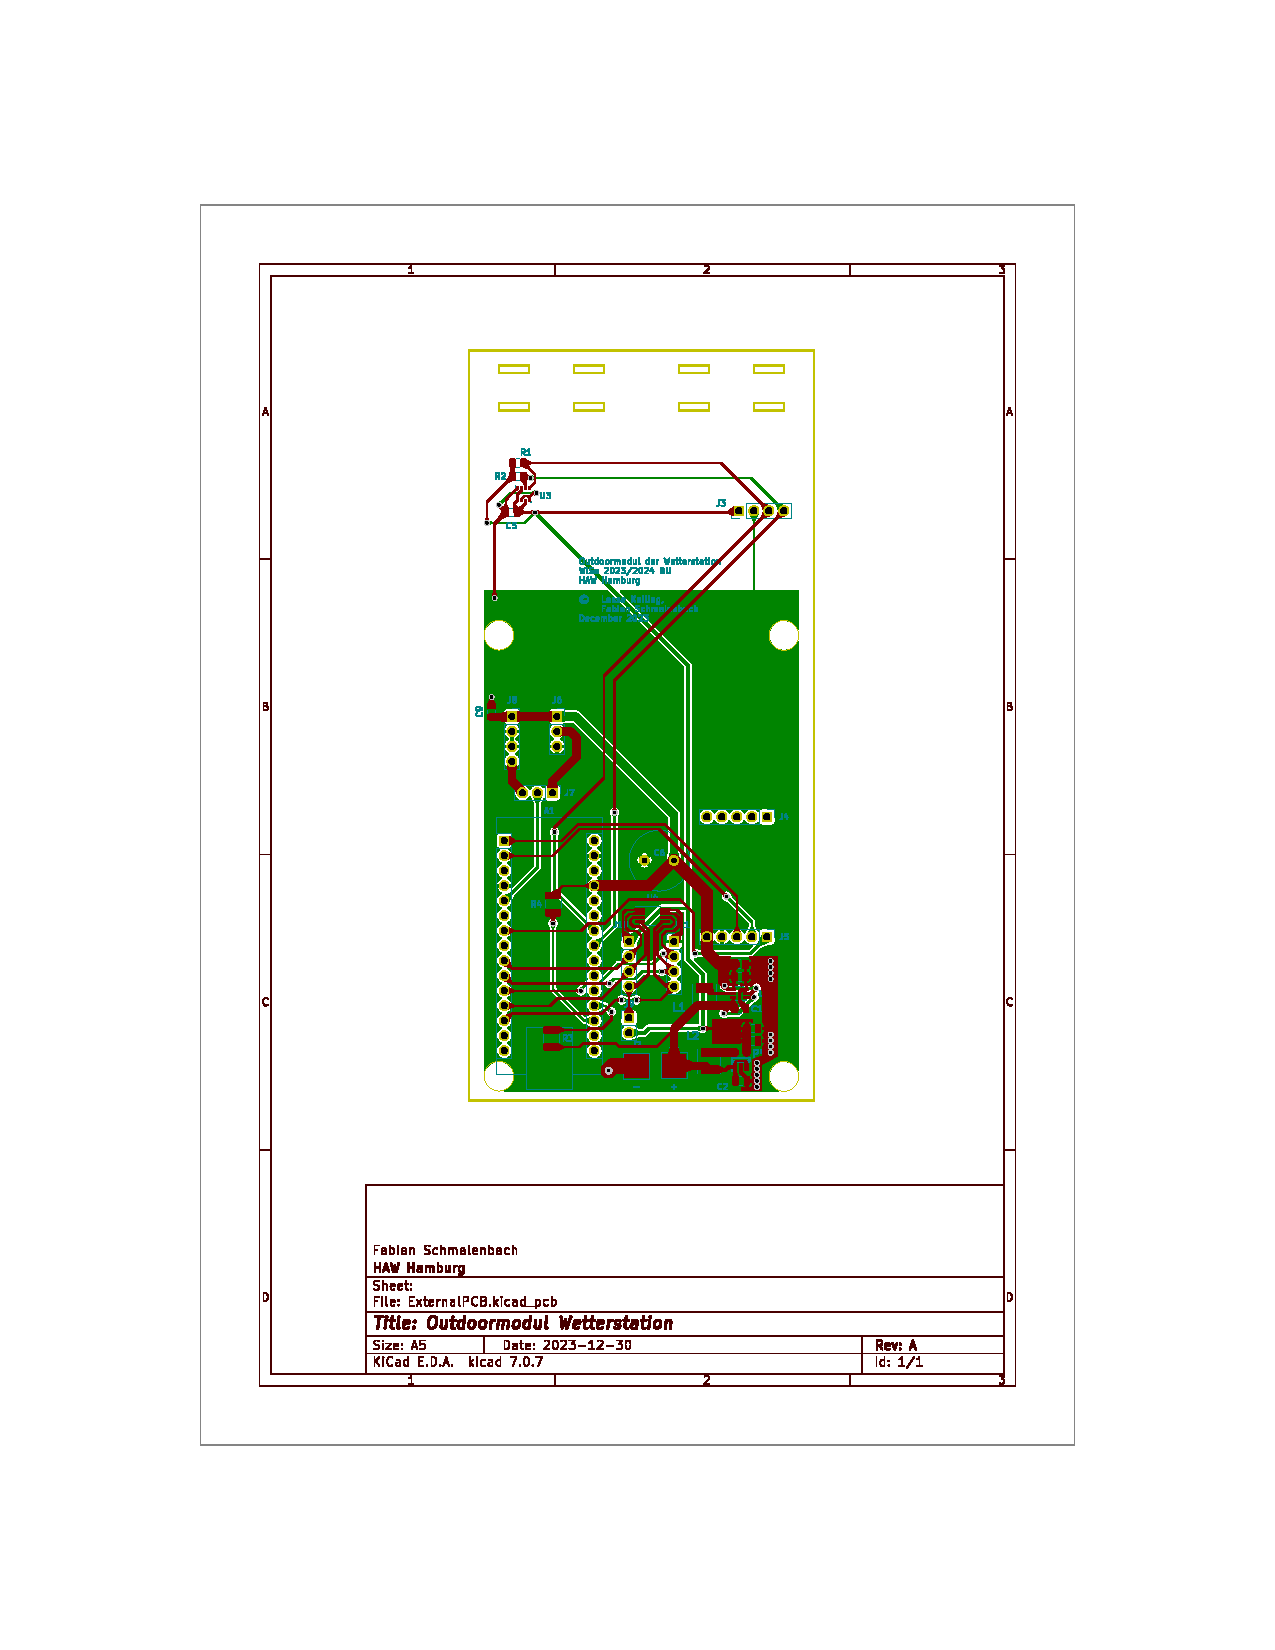
\includegraphics[scale=0.7, page=1]{PCBExtern.pdf}
  \caption{2D Ansicht des Platinenentwurfs}
  \label{pdf:platineExtern}
\end{figure}

\newpage
\subsection{3D Ansicht}

\begin{figure}[H]
  \centering
  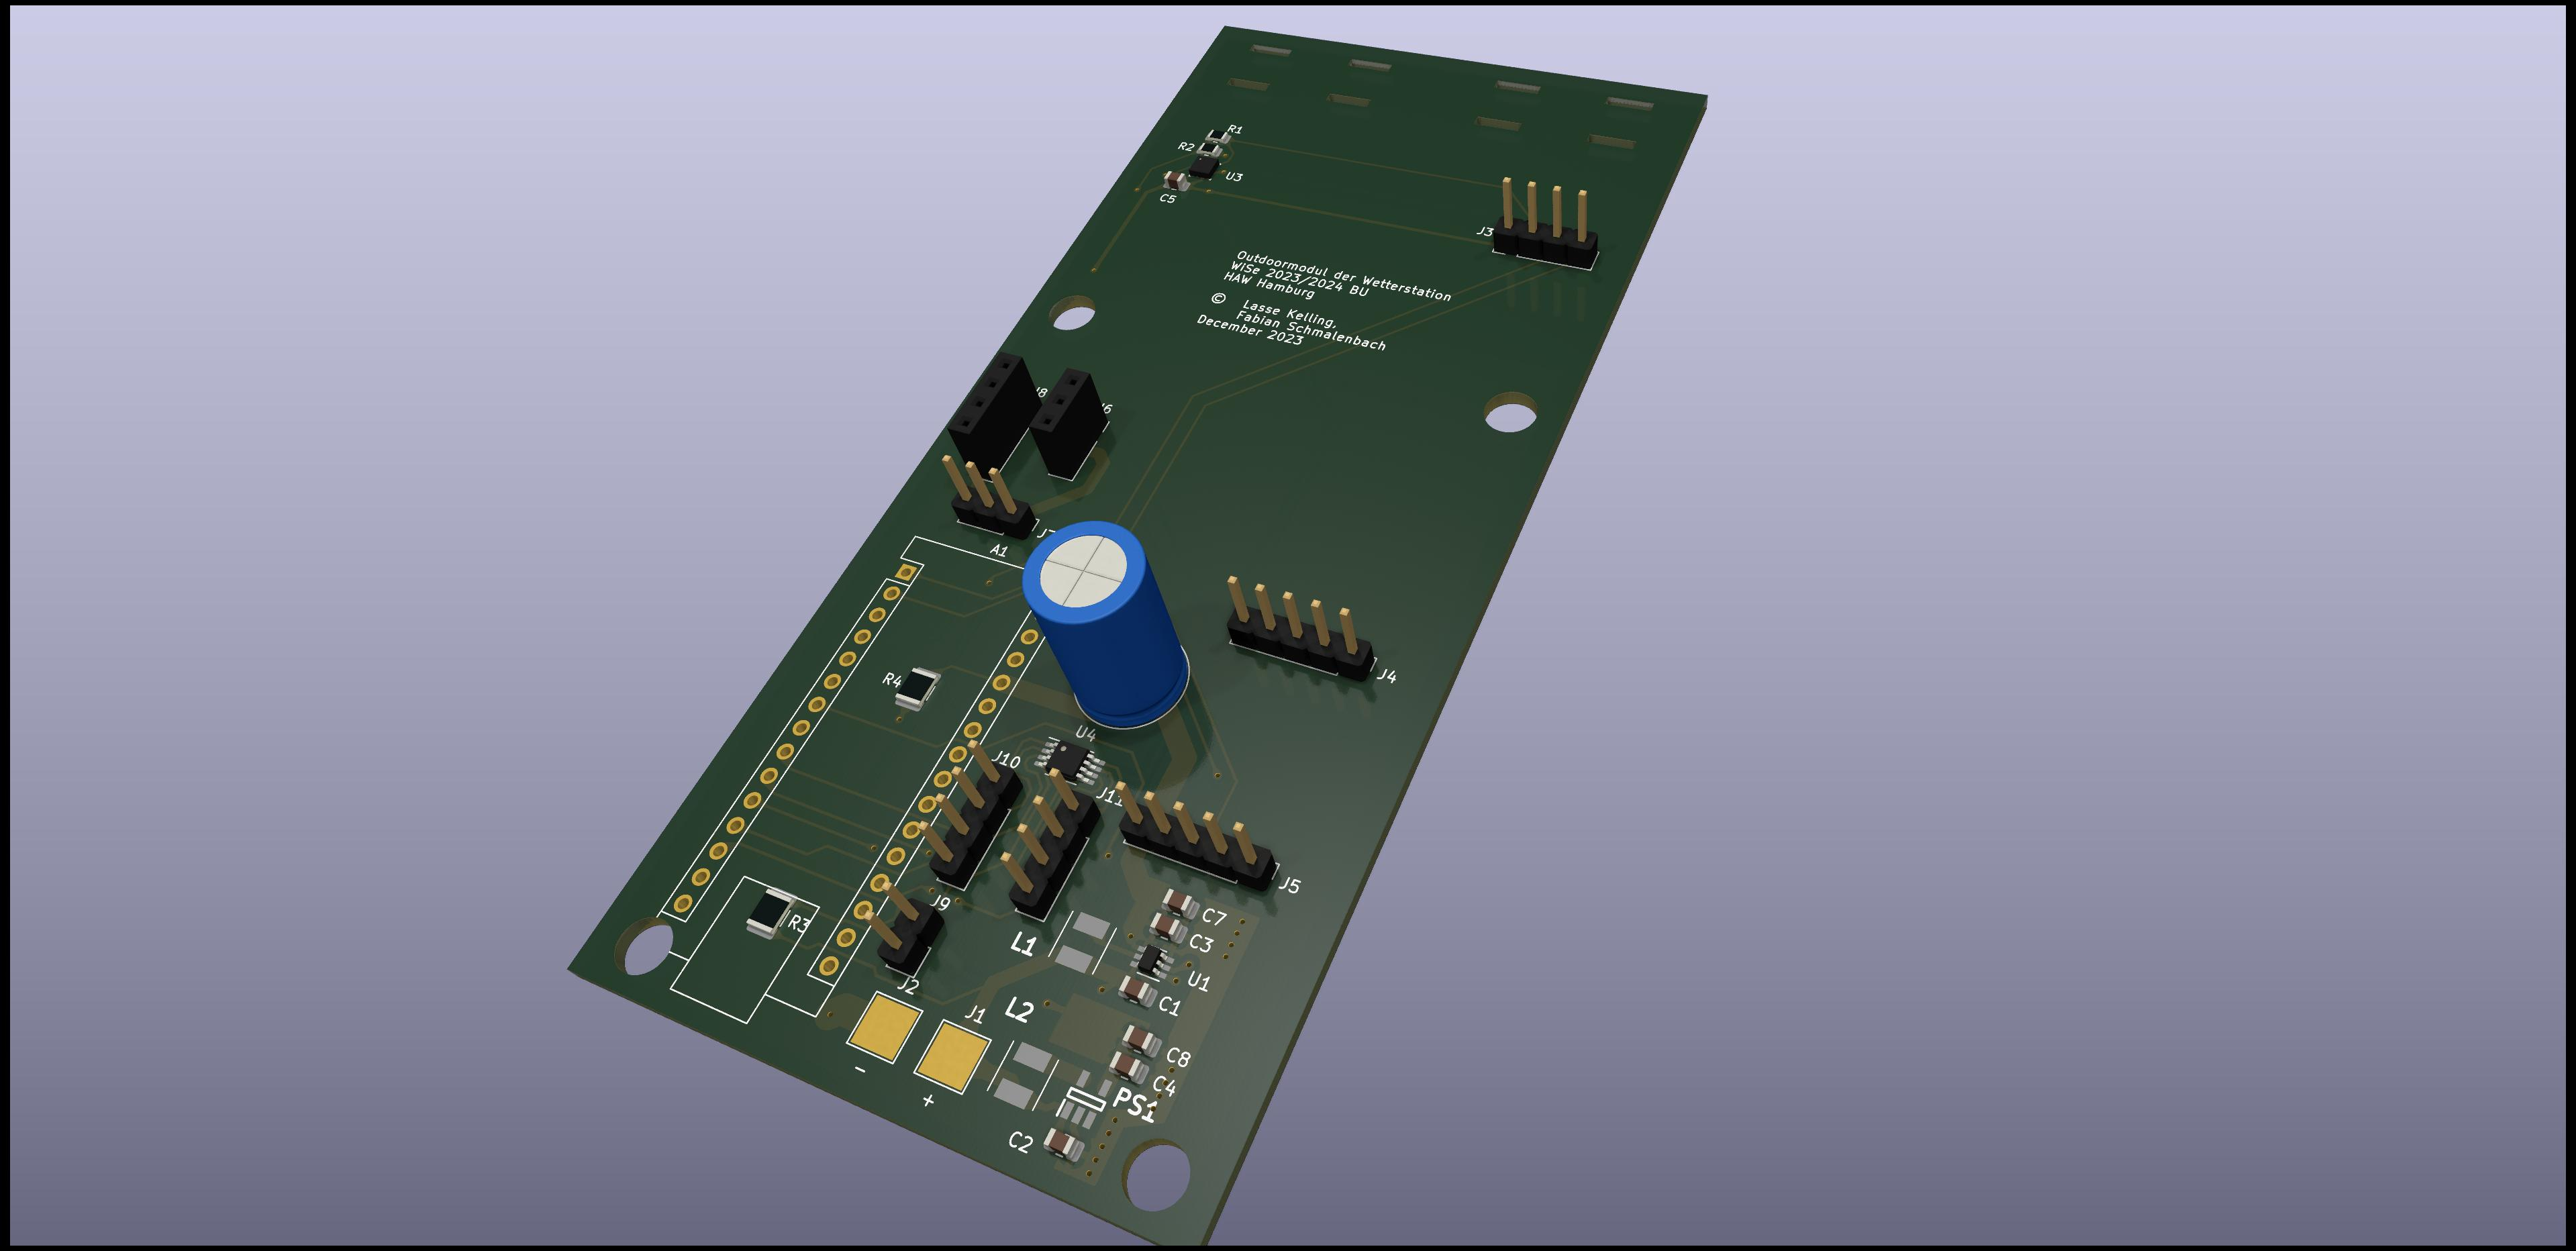
\includegraphics[width=\textwidth]{ExternalPCB3D.jpg}
  \caption{3D Ansicht des Platinenentwurfs}
  \label{fig:platineExtern3D}
\end{figure}

\newpage
\section{Ablaufdiagramm internes Sensormodul}

\newpage
\section{Schaltplan internes Modul}

\begin{figure}[H]
  \centering
  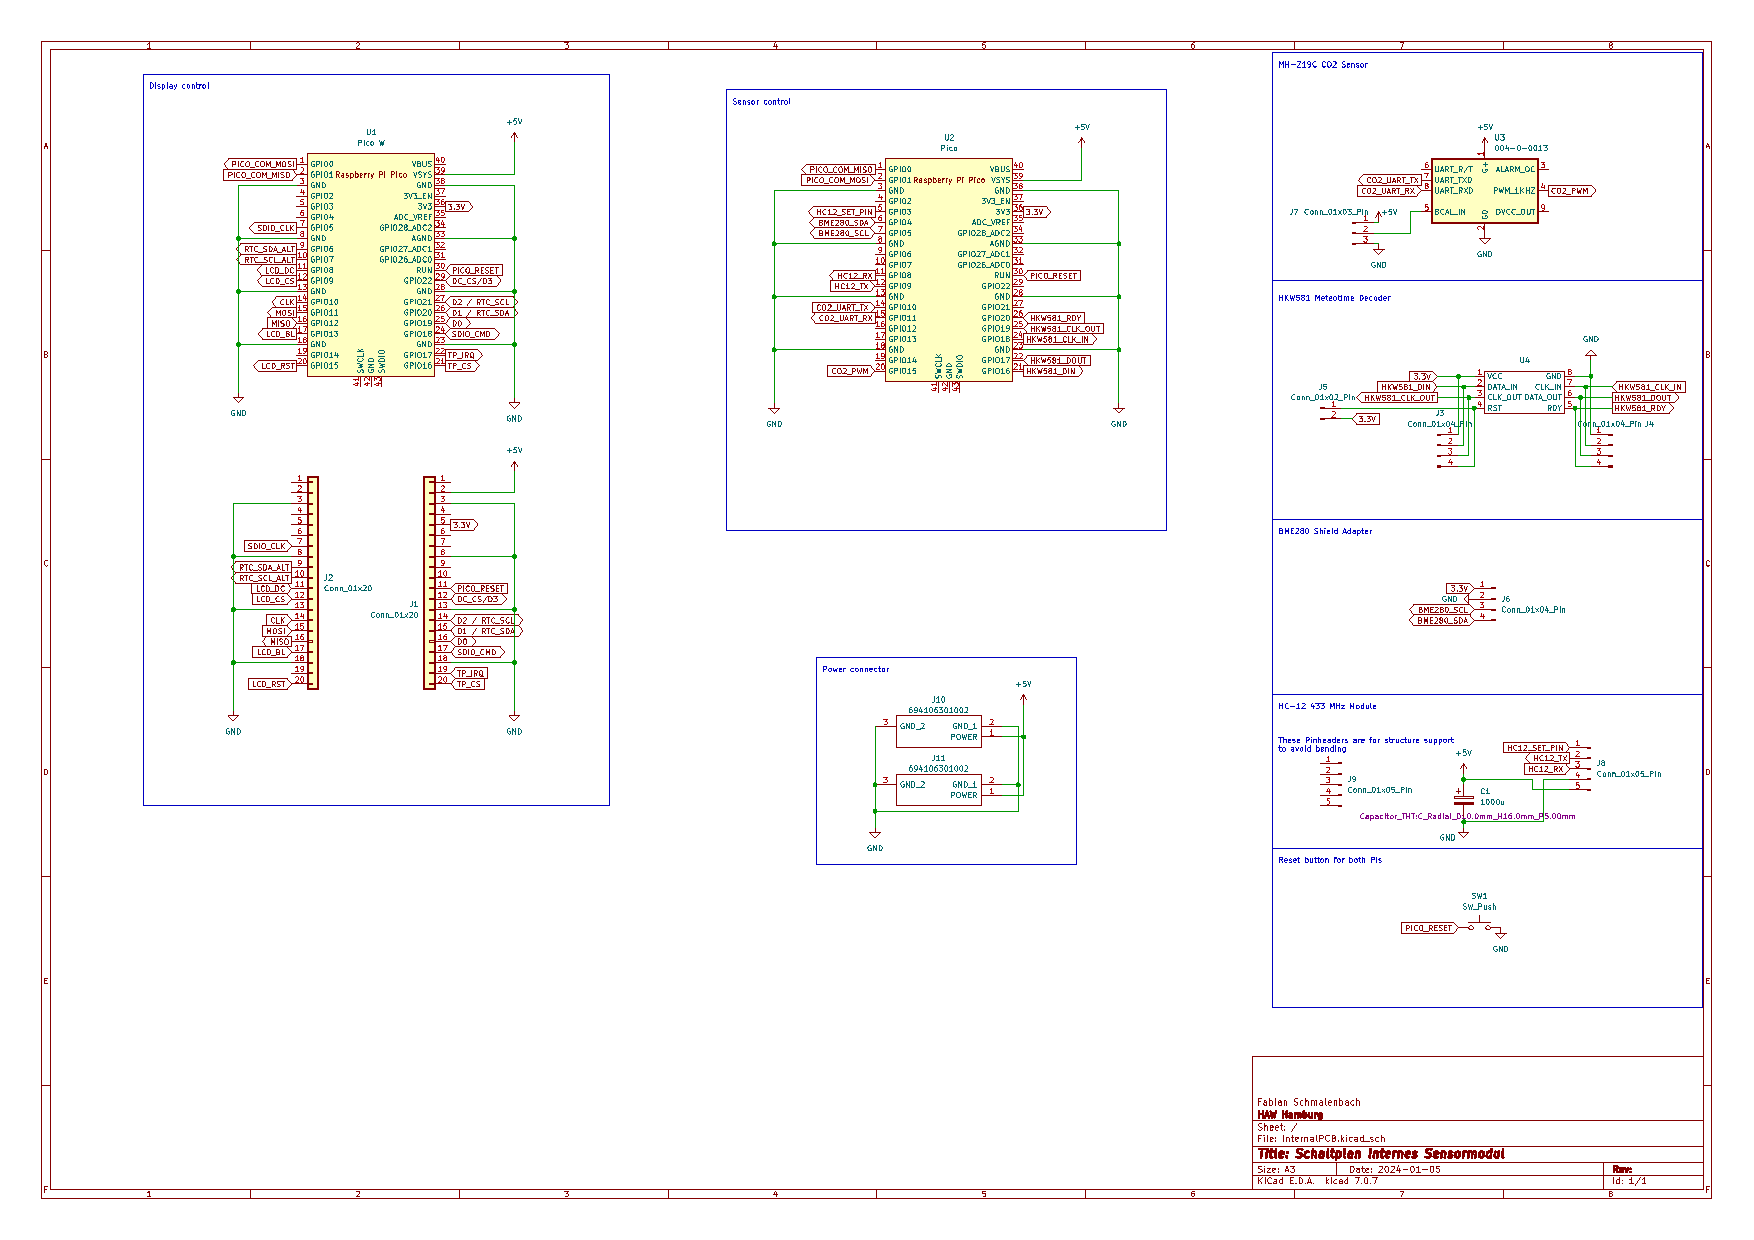
\includegraphics[scale=0.7, page=1, angle=90]{../pcbs/InternalPCB/InternalPCB.pdf}
  \caption{Schaltplan des internen Moduls}
  \label{pdf:schaltplanIntern}
\end{figure}

\newpage
\section{Platine internes Modul}

\subsection{2D Ansicht}

\begin{figure}[H]
  \centering
  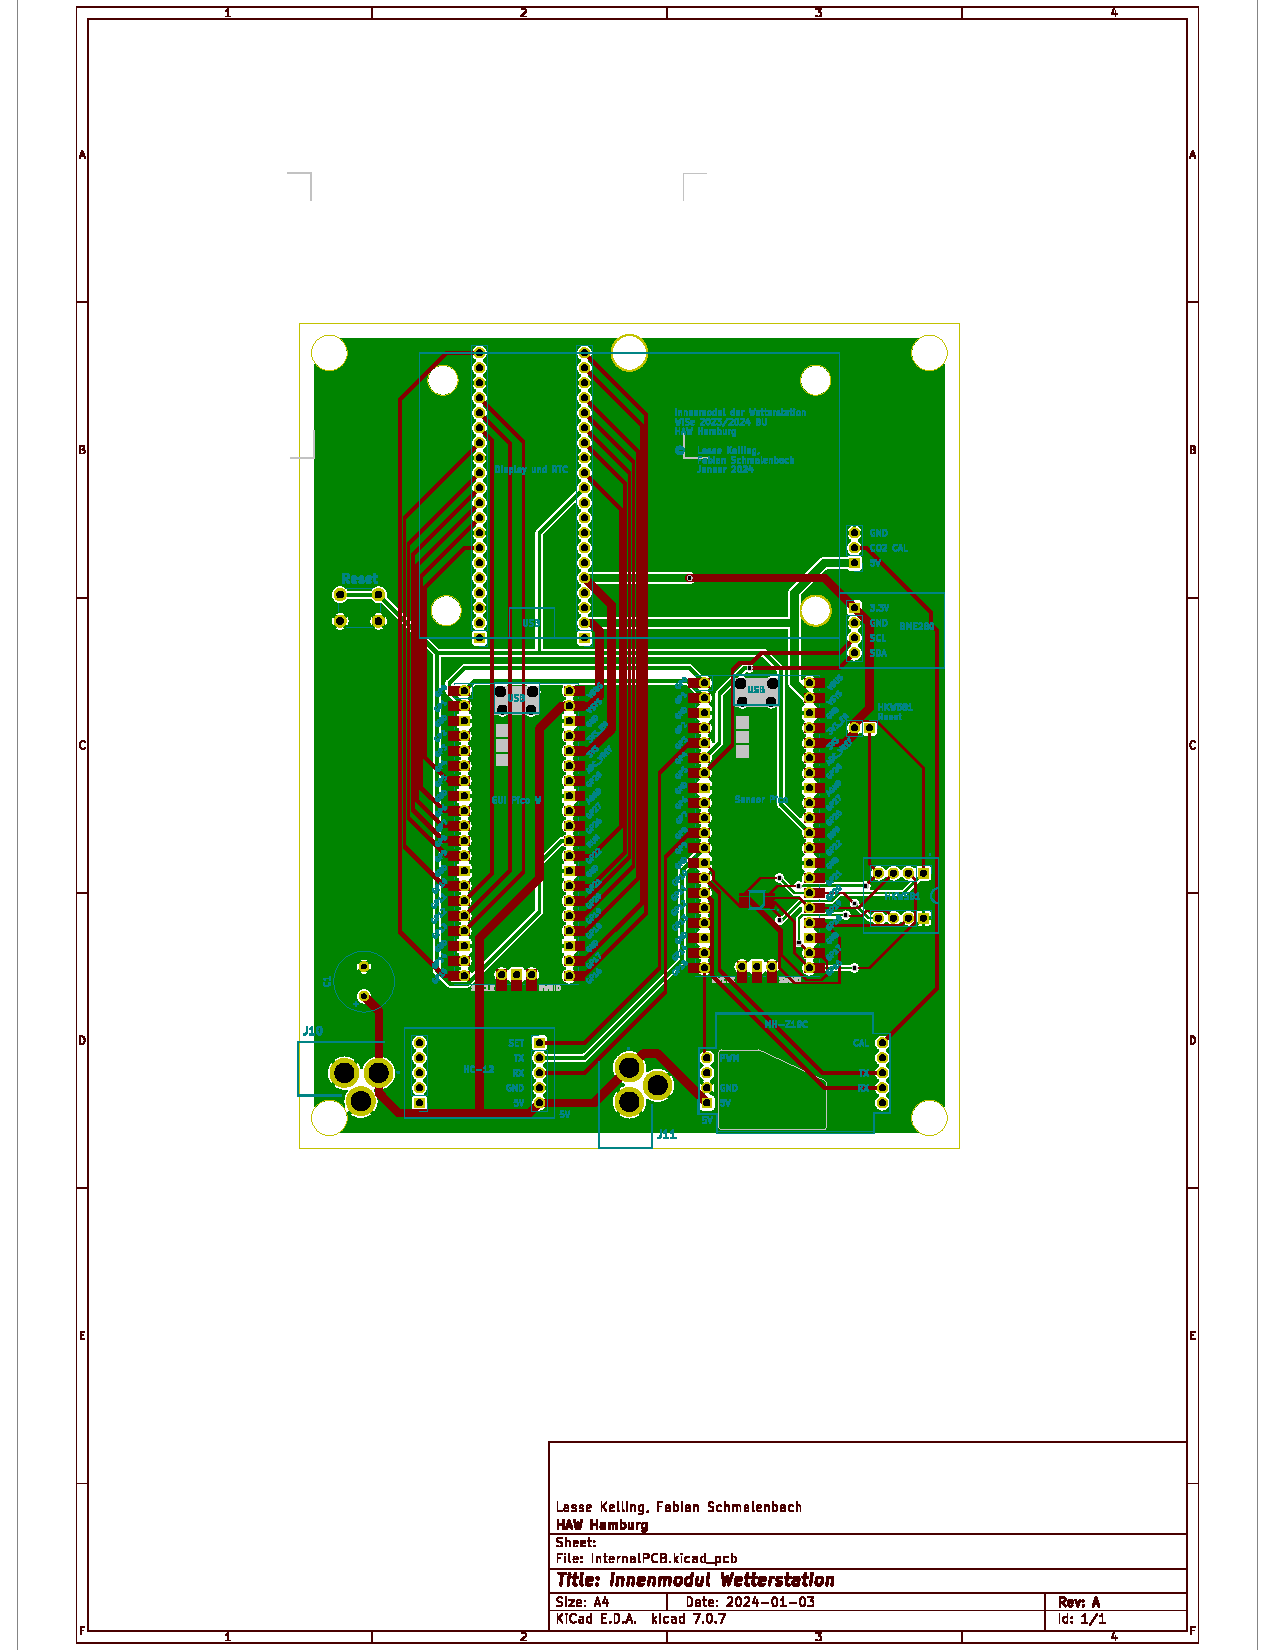
\includegraphics[scale=0.7, page=1]{PCBIntern.pdf}
  \caption{2D Ansicht des Platinenentwurfs}
  \label{pdf:platineIntern}
\end{figure}

\newpage
\subsection{3D Ansicht}

\begin{figure}[H]
  \centering
  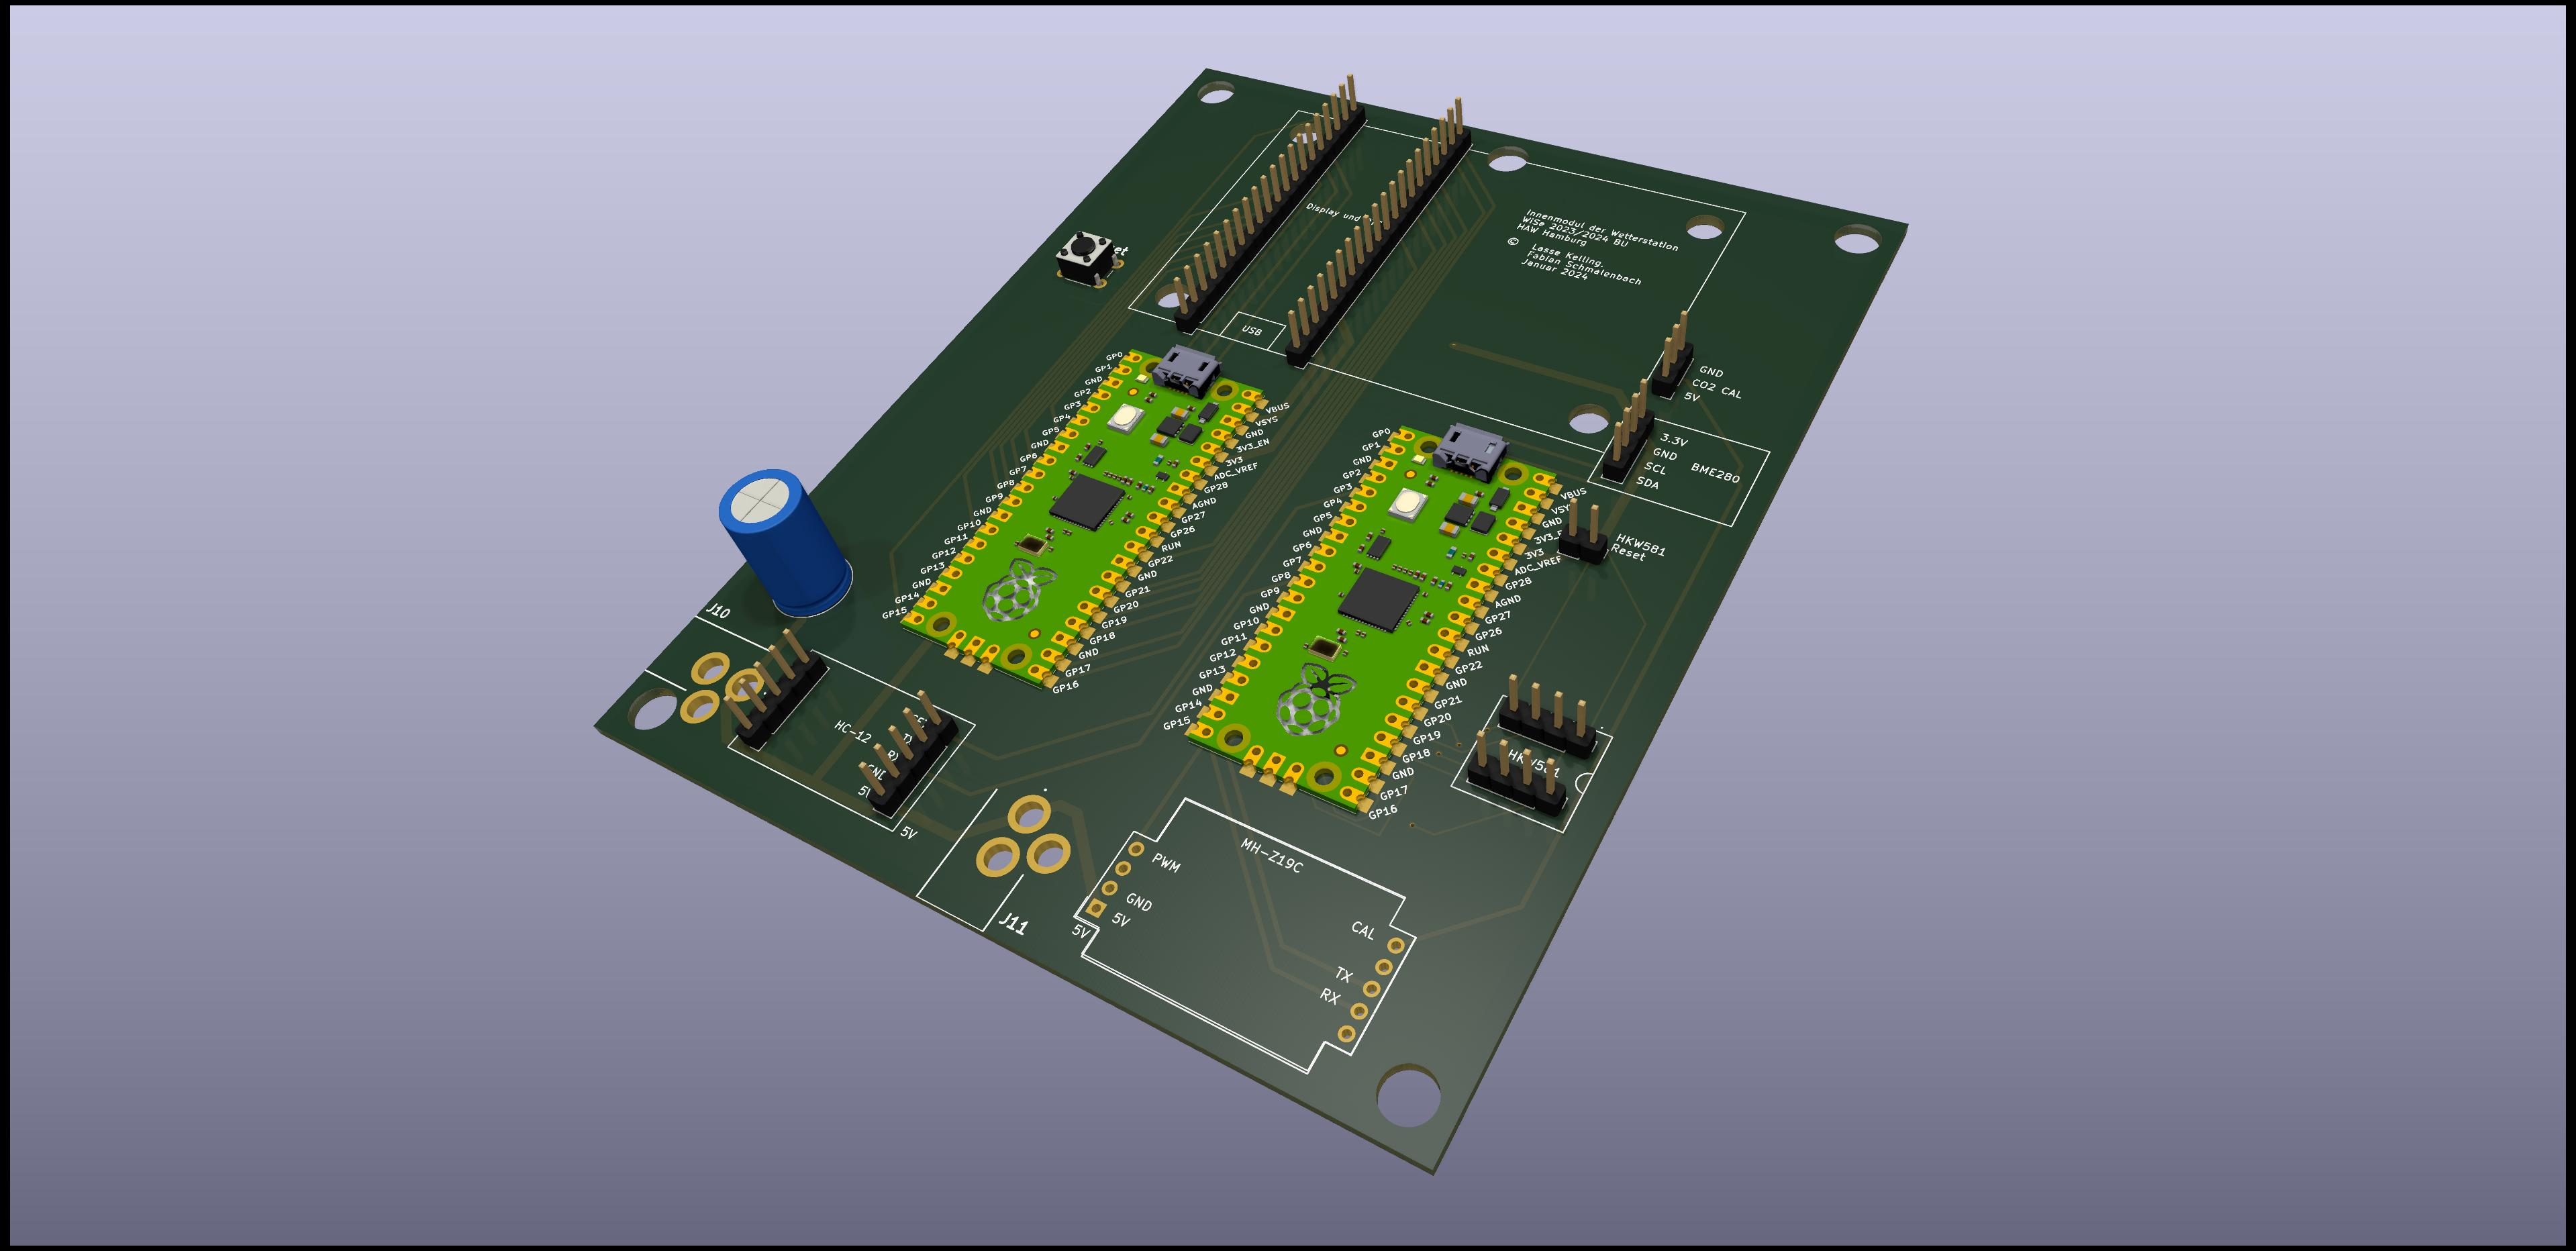
\includegraphics[width=\textwidth]{InternalPCB3D.jpg}
  \caption{3D Ansicht des Platinenentwurfs}
  \label{fig:platineIntern3D}
\end{figure}

\end{document}